\chapter{基于脉搏波的子痫前期识别分析软件系统的设计与实现}
\section{引言}
本研究此前各章中均涉及了一定的软件设计与算法设计,在这些工作的基础上,本章介绍了一款基于PPG信号的PE识别分析软件系统的设计与实现过程。在分析具体功能需求后,
选取跨平台客户端+云服务器的方案进行整体设计,以期完成以下四部分内容:PPG信号的预处理与特征计算生成;PE识别模型的本地化训练与生成;跨平台的多客户端软件设计;
云服务器端软件设计与PE识别模型的部署。本章对其中涉及的软件与算法开发设计进行了详细的介绍,同时也展示了各工作内容的实现效果,
并对软件系统简单地进行了功能性的验证与测试。

本章研究内容的框架图如\autoref{fig:frameworks6}所示。

\begin{figure}[htbp]
    \centering
    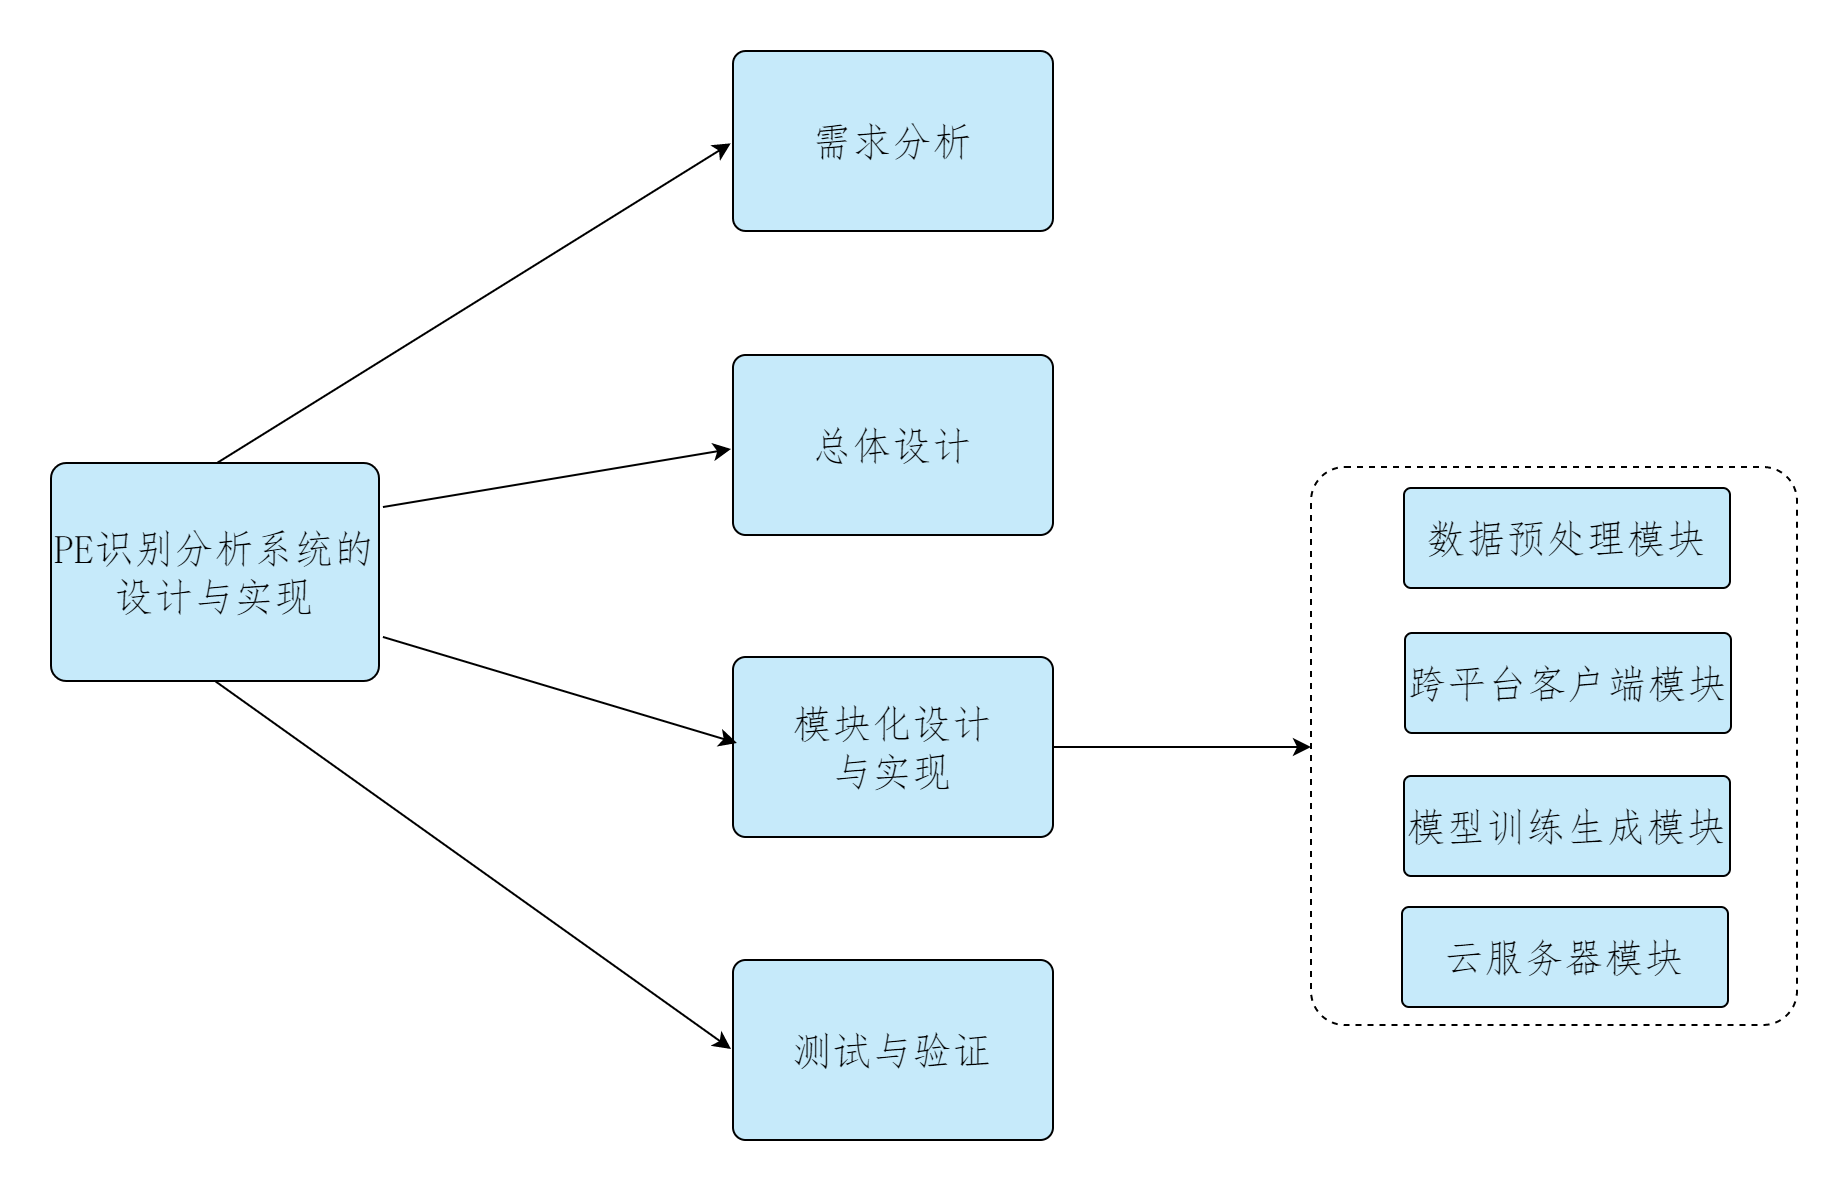
\includegraphics[width=0.9\linewidth]{software/frameworks6}
    \caption{\label{fig:frameworks6}第六章研究内容框架图}
\end{figure}

\section{需求分析}
如本研究中绪论中所介绍的,尽管移动智能医疗与可穿戴式设备已经取得了长足的发展,但现阶段PE的微型化智能化检测技术仍处于起步阶段,国内外相关研究匮乏。
而由于PE的高危害性,实现PE的早期检测识别诊断无疑可以极大地保证孕妇及婴儿的生命健康安全。因此,设计实现一款可以满足实验室研究、医院监护、社区检查、
居家监护的多应用场景的PE识别诊断软件综合系统无疑有着巨大的市场前景,具有极大的临床意义。另一方面,上述软件系统在保证完整分析功能的基础上,
应支持软件自身更新迭代导致的各种变化。这要求软件系统在开发伊始就需要进行考虑不同的开发与应用情景,引入软件开发的
代码复用与模式设计等技术,增加软件系统的健壮性与复用性\cite{Enrich2018,CJ2020}。

因此,软件系统需要满足以下具体需求,并根据实际需要,进行一定的兼容性设计:

一、核心分析功能完整

软件系统需具备完整的PE分析功能,包括不限于对原始数据进行预处理、提取计算相关特征、构建分析数据集、对数据集进行清洗、特征提取、
识别分类模型训练和生成及最后对新数据进行预测分类等。

二、可更新迭代的处理算法

在上述软件系统的核心分析功能的各环节中均会涉及到一定的处理算法,如数据预处理时的滤波检波算法、特征提取时的各种新型参数的计算算法以及识别模型的机器学习训练生成算法等。
软件系统需要支持对以上算法的更新与迭代,避免由于算法的调整、切换、更新、迭代等操作引发大量的代码修改与重构等问题的出现。

三、可动态调整的识别模型

在第五章已经介绍过,多种机器学习算法均在PE的识别分析中得到了应用。软件系统需要支持对这些由不同算法生成的不同识别模型的切换,
针对需要预测的新数据,保证返回对应模型的预测结果。

四、有效的数据管理

由软件系统的核心功能分析可知,除最基本的原始数据外,系统还需要对基于原始数据的二次提取特征参数、数据集划分结果、PE识别模型的训练参数及模型本身等多种数据进行管理。
如何高效、有序的管理各类原始数据及中间数据也是软件系统需要解决的问题之一。

五、云服务器+跨平台客户端

软件系统需要充分考虑到多种满足在实验室研究、医院监护、社区检查、居家监护多种场景下不同的使用需求。因此,云服务器+客户端无疑是最优的解决方案,而考虑到智能便携式设备的普及,
PC端与移动端均需开发对应的客户端。

六、完备的日志记录

软件系统需要具有完备的日志记录功能,方便在开发或部署到生产环境中之后,随时定位、调试可能出现的问题。由于软件系统模块繁多、功能齐全,如果没有完备的日志记录功能,
软件系统的debug过程将举步维艰,同时,也很难评估软件系统的运行状态。

七、数据源兼容性

软件分析系统的使用的原始数据可能来自多种硬件采集设备自行采集或公开数据库。对于采集得到的数据,不同硬件设备使用的电子元器件、传感器等在性能参数上的区别可能导致
采集得到的数据在信号质量、采样率、分辨率及数据存储与解析格式等方面均存在差异。而由数据库得到的数据,其字段信息也极容易出现差异。保持对不同数据源的兼容性
也是软件分析系统需要重点解决的问题之一。

八、其他拓展性

基于本研究此前章节相关内容,软件分析系统使用PPG信号作为原始数据输入。但随着高性能的数据采集设备的普及,同时使用多通道多参数生理信号(如ECG、BCG、EEG)
也存在着联合分析的可能,需要软件分析系统进行一定的兼容性设计。此外,尽管软件分析系统是为PE的识别分析为初衷进行设计,其核心分析功能可作为类似研究的参考模板,
软件分析系统在进行设计时也可以考虑整体的移植性。

\section{总体设计}

根据上小节中需求分析的相关内容,最终实现的软件分析系统按照低耦合、高拓展的原则进行了模块化、功能化的设计,
每一模块只处理某一类特定任务,以实现功能高内聚性,并保持模块间的松耦合性。

一、模块化设计

软件分析系统整体设计框图如\autoref{fig:scas}所示。上小节中提及的软件系统的核心分析功能被拆分为四个独立的功能模块分别实现,以下为具体介绍。
\begin{figure}[htbp]
    \centering
    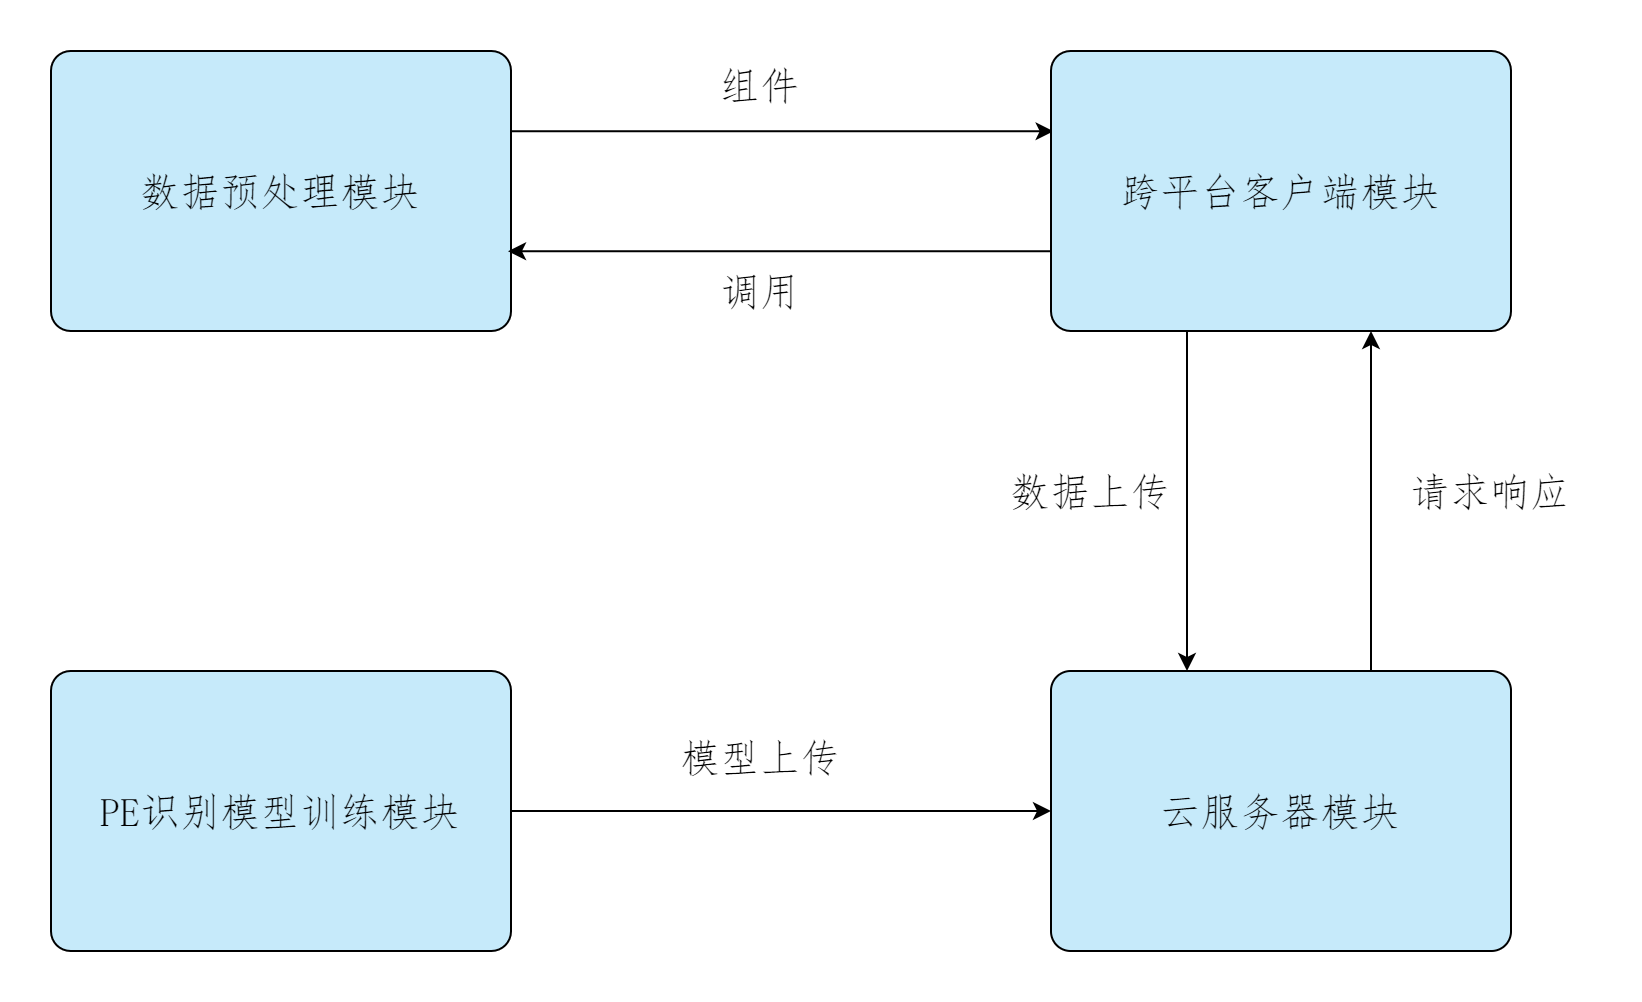
\includegraphics[width=.6\linewidth]{software/scas}
    \caption{\label{fig:scas}软件分析系统的多模块设计框架图}
\end{figure}

1、数据预处理模块

数据预处理模块主要负责从原始PPG信号中提取数据特征,包括数据的读取、PPG信号的滤波降噪、波形的检测识别、特征定义及计算等处理任务。
数据预处理模块的各项处理算法或处理步骤需具有稳定性,不依赖具体部署的平台或应用场景。在此前第三章中介绍过的SCD算法也在数据预处理模块涵盖范围内。

2、跨平台客户端模块

为在多种平台下使用本软件系统,跨平台客户端模块需要完成所需操作平台下的客户端的开发。上述数据预处理模块直接在客户端模块中得到调用,PPG波形的特征数据经客户端
经由互联网被发送至云服务器端进行处理分析,云服务器的处理分析结果也会经由互联网发送返回给客户端进行展示。

3、PE识别模型训练生成模块

在获取客户端发送来的数据后,PE识别模型训练生成模块需要选择合适的机器学习算法基于这些输入数据训练生成PE识别模型,模型在训练过程中所使用的具体数据集、初始参数及调整优化后
的超参数需要同时被记录保存。生成得到的PE识别模型最终需要被部署在云服务器上,为后续新数据进行预测分析。

4、云服务器模块

云服务器模块负责管理由客户端发送来的数据信息、管理系统具体PE识别模型。当客户端发来新的数据并请求分析时,云服务器模块从客户端发送来的参数信息中确定具体使用的识别模型,
将数据交由对应的模型进行分析后,将分析结果返回至发出请求的具体客户端。

二、设计原则的应用

为使具有以上功能的多模块化软件系统的开发能顺利进行,在开发过程中必须借助计算机软件开发领域的相关思想,遵循一定的开发原则。

1、面向对象编程

面对对象编程(Object Oriented Programming,OOP)是一种计算机编程架构,尽可能模拟人类的思维方式,使得软件的开发方法与过程尽可能接近人类认识世界、
解决现实问题的方法和过程。OOP使得描述问题的问题空间与问题的解决方案空间在结构上尽可能一致,把客观世界中的实体抽象为问题域中的对象。
借助OOP的抽象、继承、多态等特性,可以简化复杂的编程过程,使软件开发的逻辑更为简单。

2、设计模式

设计模式(Design Pattern,DP)是计算机软件设计中对某些特定问题的优化解决方案的总结。DP是一套被反复使用、多数人知晓的、经过分类编目的、代码设计经验的总结。
在程序开发过程中使用设计模式,可重用代码、让代码更容易被他人理解,保证代码可靠性的同时也增加了程序的重用性。

三、编程语言与开发环境

软件系统各模块所使用的编程语言与开发环境工具如\autoref{tab:ides}所示,模块所使用的一些重要组件或开源库也在表格中进行了说明。

\begin{longtblr}
    [
        theme                   = {zju},
        caption                 = {不同模块使用的编程语言与开发环境汇总},
        label                   = {tab:ides},
    ]
    {
        width                   = \linewidth,
        colspec                 = {X[1,c,m]X[1.8,c,m]X[1,c,m]X[1,c,m]X[2,c,m]X[1.5,c,m]X[1.5,c,m]},
        hline{1,Z}              = {\thickline},
        hline{2}                = {\thinline},
        rowhead                 = 1,
        row{3,4,6}              = {bg=\oddcolor}, 
        row{2,5}                = {bg=\evencolor},
        row{1}                  = {font=\headfont,bg=\headcolor},
        row{2-Z}                = {font=\nonheadfont},
        cell{3}{1-2}            = {r=2,c=1}{c,m},
    }
    序号 & 模块 & 平台 & 开发语言 & 版本 & 开发工具 & 其他组件或库 \\
    1 & 数据预处理 & / & Java & OpenJDK(16.0.2) & VS Code & / \\
    2 & 客户端 & PC & Java & OpenJDK(16.0.2) & VS Code & / \\
    2 & 客户端 & Android & Java & Android Studio default JDK(11.0.12)  & Andoird Studio & / \\
    3 & 模型训练 & / & Python & 3.9.7 & PyCharm & Sklearn \\
    4 & 云服务器 & / & Python & 3.9.7 & PyCharm & Django、Sklearn \\
    
\end{longtblr}

软件系统的数据预处理模块与客户端模块使用Java语言开发完成。
作为一种高级语言,Java兼具解释型编程语言与编译型编程语言的特性,是目前最流行的面向对象语言之一\cite{Li2015}。
除一般面向对象编程语言的抽象继承等特性外,Java还支持抽象类、接口等设计,可以满足上述此前需求分析中的各项具体内容。
Java具有出色的跨操作系统平台特性,可以实现一次编译、多处使用。除PC端外,Java同时也是移动操作系统Android的主力开发语言之一\cite{android}。
鉴于Java的种种优点,因此,软件系统的数据预处理模块与PC客户端模块最终选择了Oracle开源版本的OpenJDK(16.0.2,GPLv2协议)\cite{openjdk}在VS Code集成开发环境
(Integrated Development Environment,IDE)下开发完成;
而Android客户端则选择了Android Studio作为IDE,使用Android Studio自带的Java版本(11.0.12,Apache协议)完成开发。


软件系统的模型训练模块与云服务器模型使用Python语言开发完成。
Python是一种高层次的结合了解释性、编译性、互动性和面向对象的脚本语言,是近年来最为流行的编程语言。
Python开源、免费、易学,也具备极强的可移植性,可以非常方便地部署在不同的操作系统与平台下。
此外,Python有着非常丰富的库组件,包括科学计算与人工智能领域极为有名的NumPy、SciPy、Sklearn与TensorFlow等组件。
因此,软件系统的模型训练与云服务器模块均选择了开源的Python(3.9.7,GPL协议)在PyCharm IDE下开发完成。
此外,云服务器模块还选取了基于Python的Django为Web框架完成服务器端相应功能的开发,选择了MySQL作为数据存储的数据库。

\section{模块设计}

针对需求分析中提出的多项具体要求,本小节将具体介绍总体设计中确定的四个模块的设计与开发过程。
\subsection{数据预处理模块}

数据预处理模块整体的处理流程如\autoref{fig:preprocess2}所示。下面依次介绍流程中各步骤的详细设计。
\begin{figure}[htbp]
    \centering
    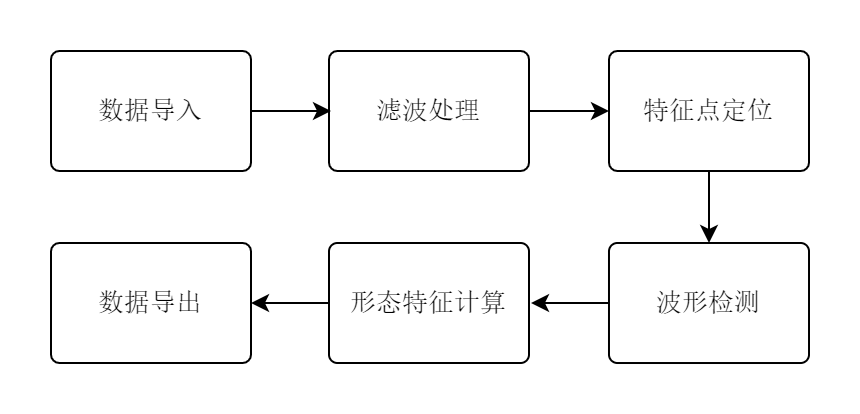
\includegraphics[width=.65\linewidth]{software/preprocess}
    \caption{\label{fig:preprocess2}数据预处理模块流程图}
\end{figure}

一、数据导入

为保持对来自不同硬件设备采集的原始数据保持读取的兼容性,软件系统将数据读取过程进行了抽象,如\autoref{fig:template}所示。
数据读取的过程被设计为一个抽象基类,其中的读取方法被设计为一个抽象方法,该方法只定义了函数名,而不进行具体实现。
当需要读取具体来源的数据时,必须重新定义该基类的一个子类,并在子类中详细实现具体的读

\begin{figure}[htbp]
    \centering
    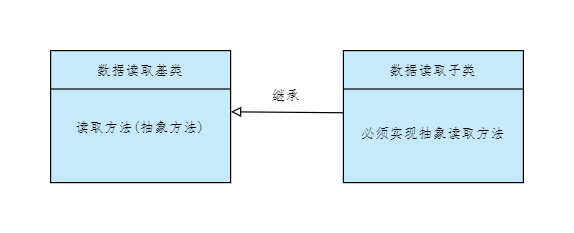
\includegraphics[width=.7\linewidth]{software/read}
    \caption{\label{fig:template}数据导入的设计}
\end{figure}
\begin{figure}[htbp]
    \centering
    \subfigure[GE B650监护仪]{
    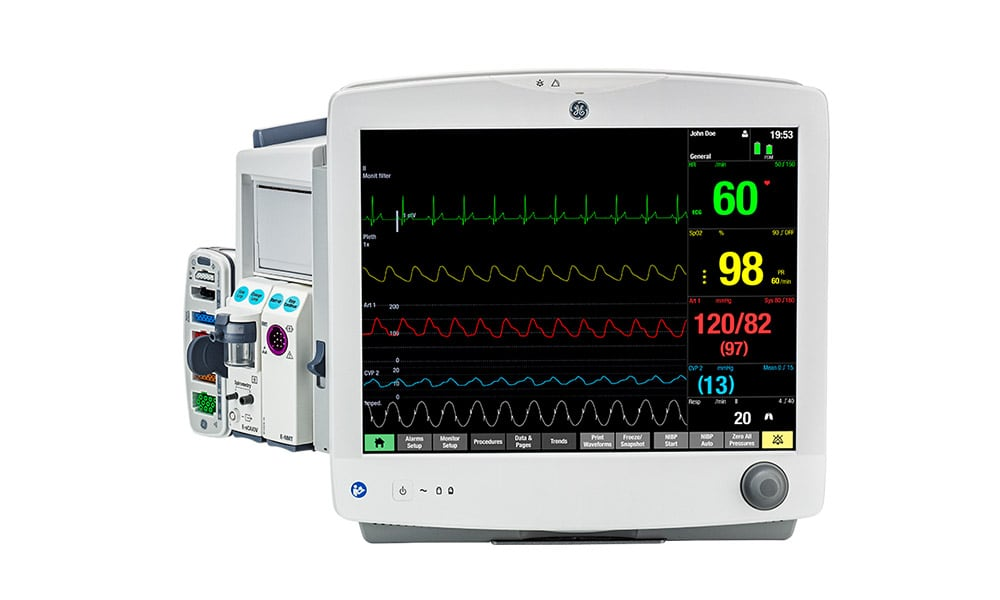
\includegraphics[width=5.5cm]{pulse_preprocess/monitor1}
    }
    \quad
    \subfigure[迈瑞ePM 15M生理信号监护仪]{
    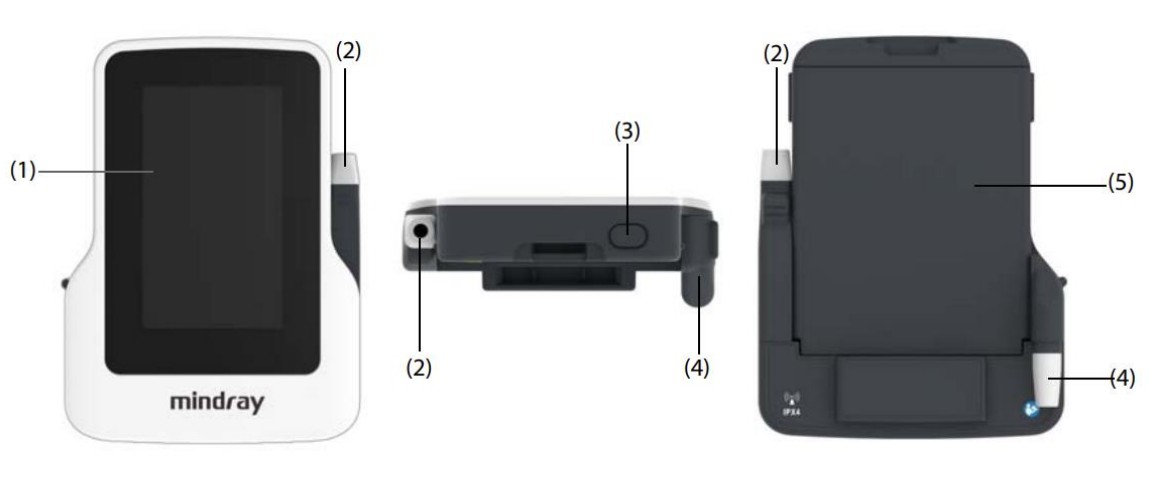
\includegraphics[width=5.5cm]{software/ep20}
    }
    \quad
    \subfigure[研究团队自研的多生理参数采集设备]{
    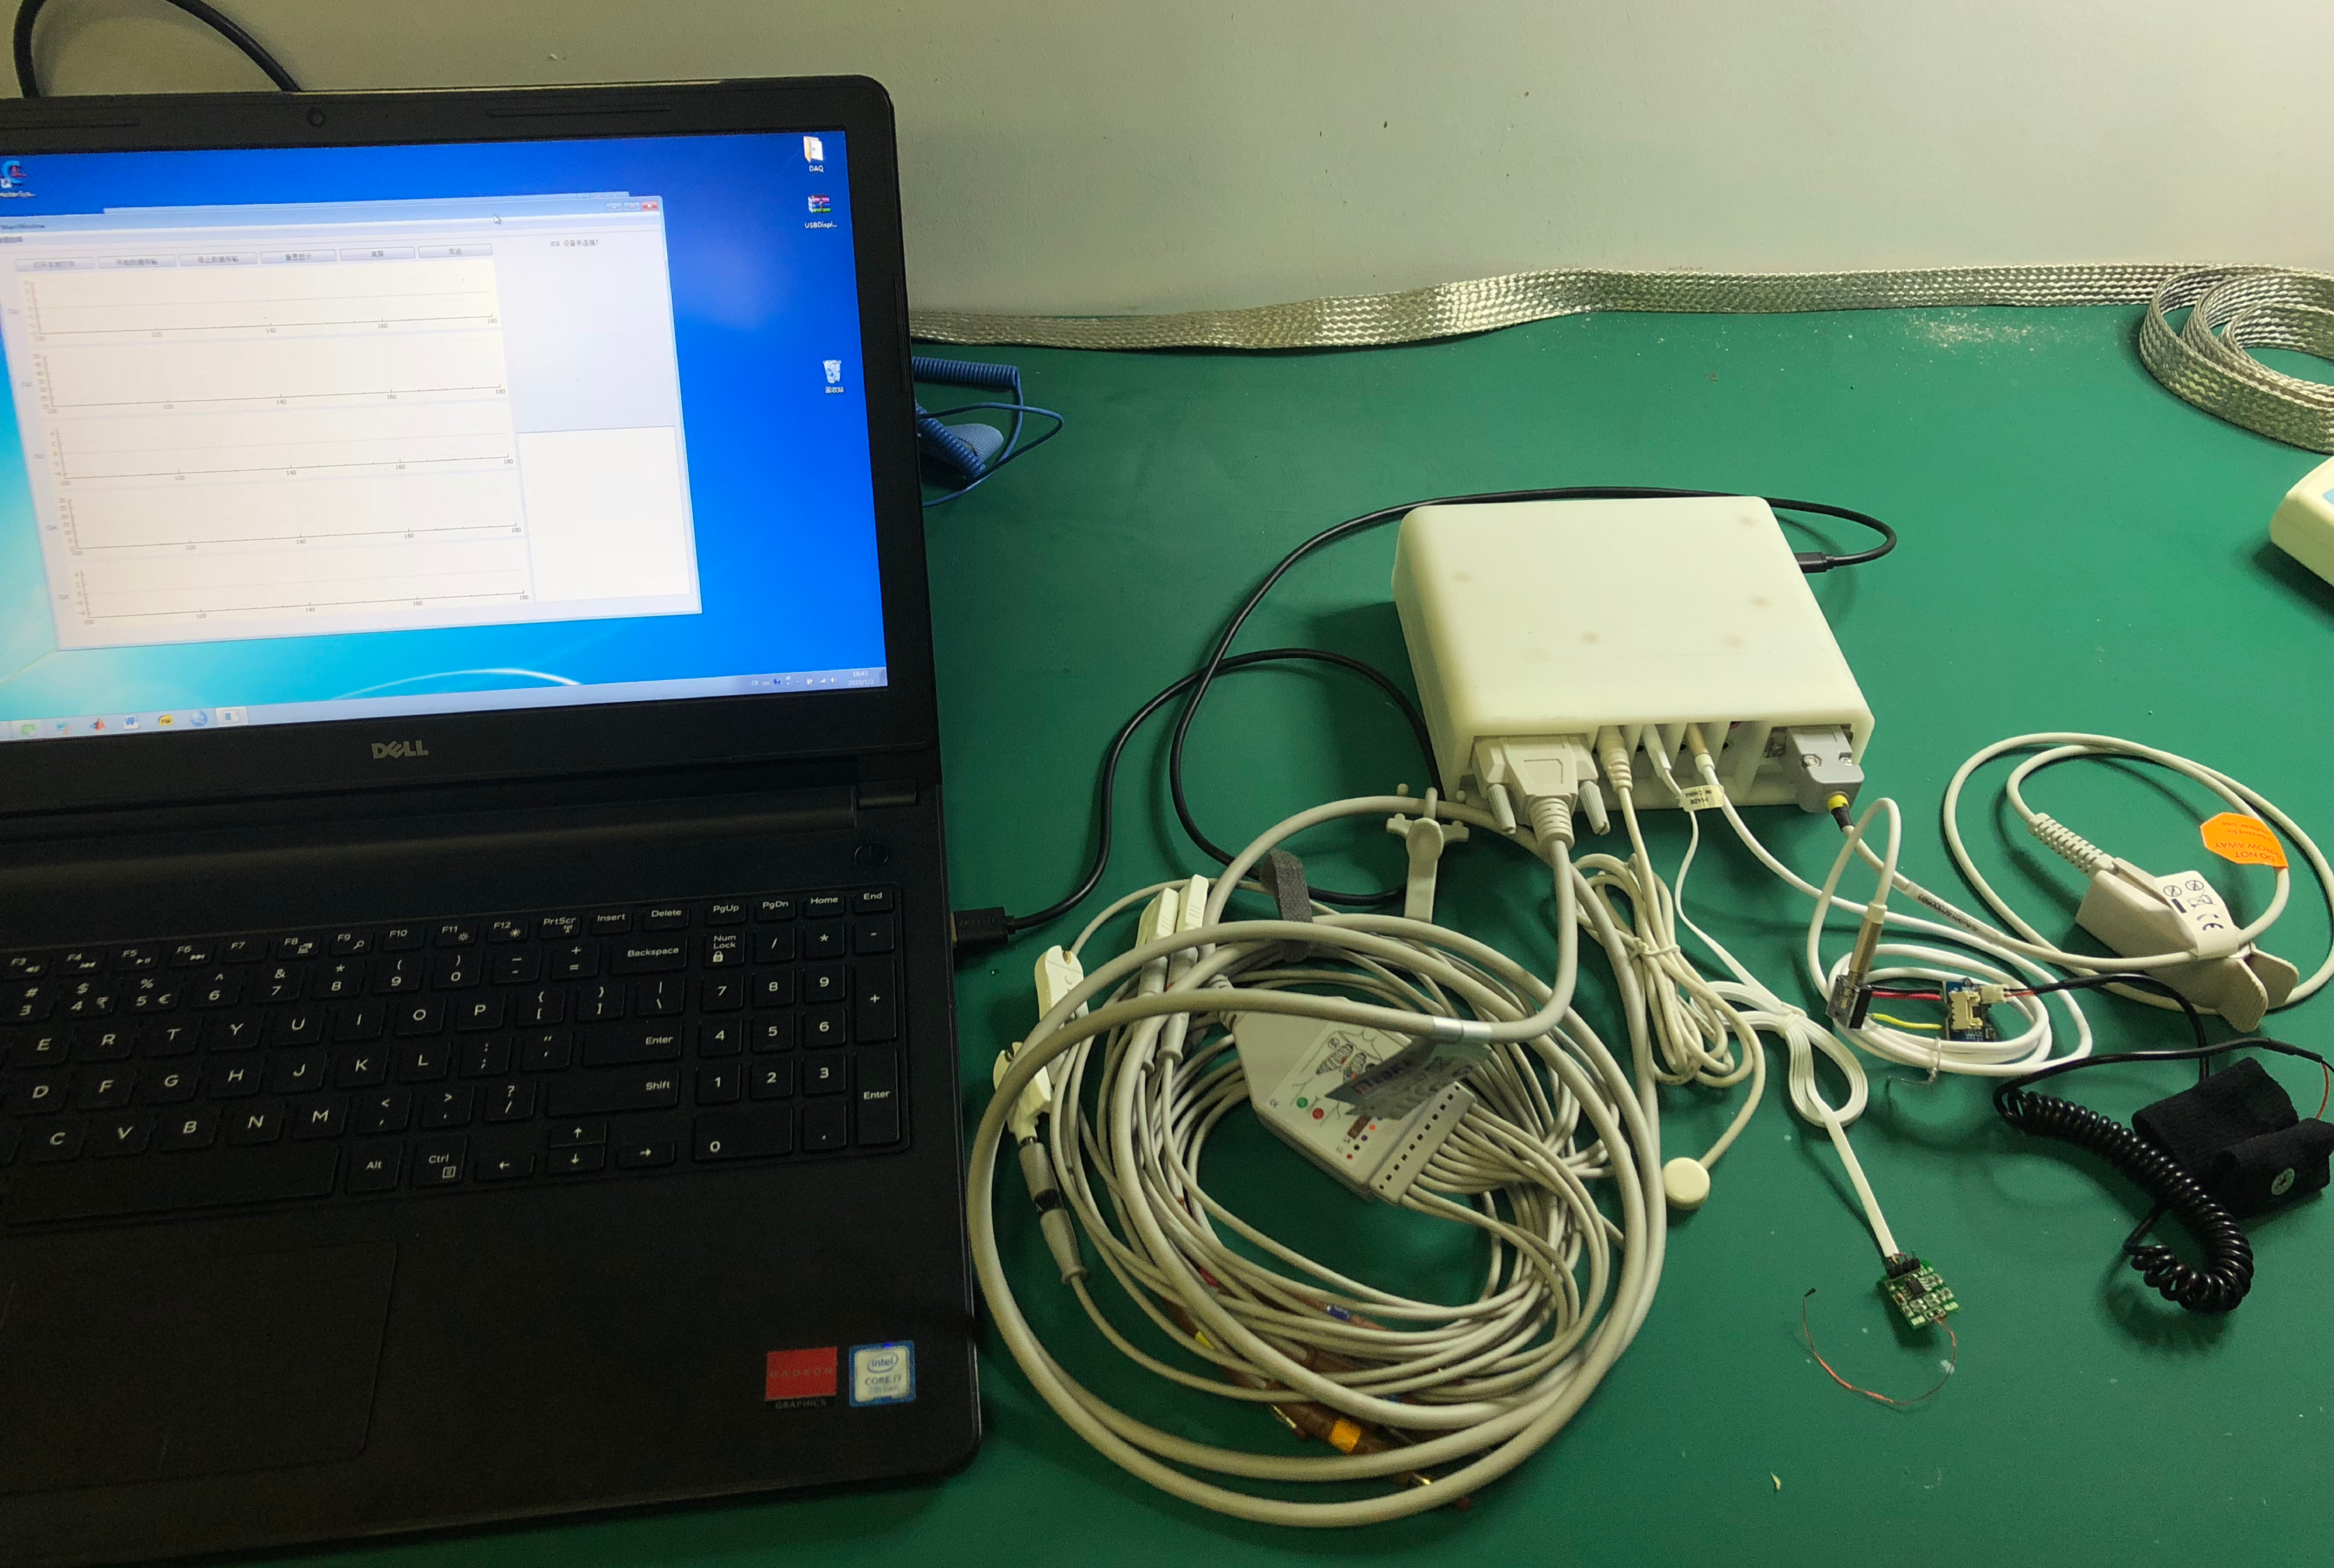
\includegraphics[width=5.5cm]{software/SystemCon}
    }
    \caption{\label{fig:data_sources}软件系统目前支持的几款硬件设备}
\end{figure}
\noindent
取方法。
此时,由硬件差异、数据格式等原因导致的读取方法的差异可以在该抽象基类的不同子类中实现。

以上机制延迟实现了读取的具体处理过程,隔离了数据读取功能对系统其他功能的影响,也保证了系统整体的灵活性。
在这种设计下,目前软件系统已经支持对GE、迈瑞ePM 15M生理信号监护仪等多种医用监护仪导出的数据的读取,
同时也支持研究团队自研的多生理参数采集设备的数据读取,如\autoref{fig:data_sources}所示。

二、滤波处理

在对生理信号的进行数字滤波时,一般会涉及多种类型的数字滤波器甄选。同时,每种滤波器也会有相应的可调参数。
因此,性能最佳的滤波器的选择往往需要对多种滤波器调参后综合测评后才能判别,软件分析系统需要能在多种滤波器之间灵活切换。
软件系统使用了DP中的模板方法(Template Method)对这一过程进行了设计\cite{Enrich2018},这一过程如\autoref{fig:template2}所示。
\begin{figure}[htbp]
    \centering
    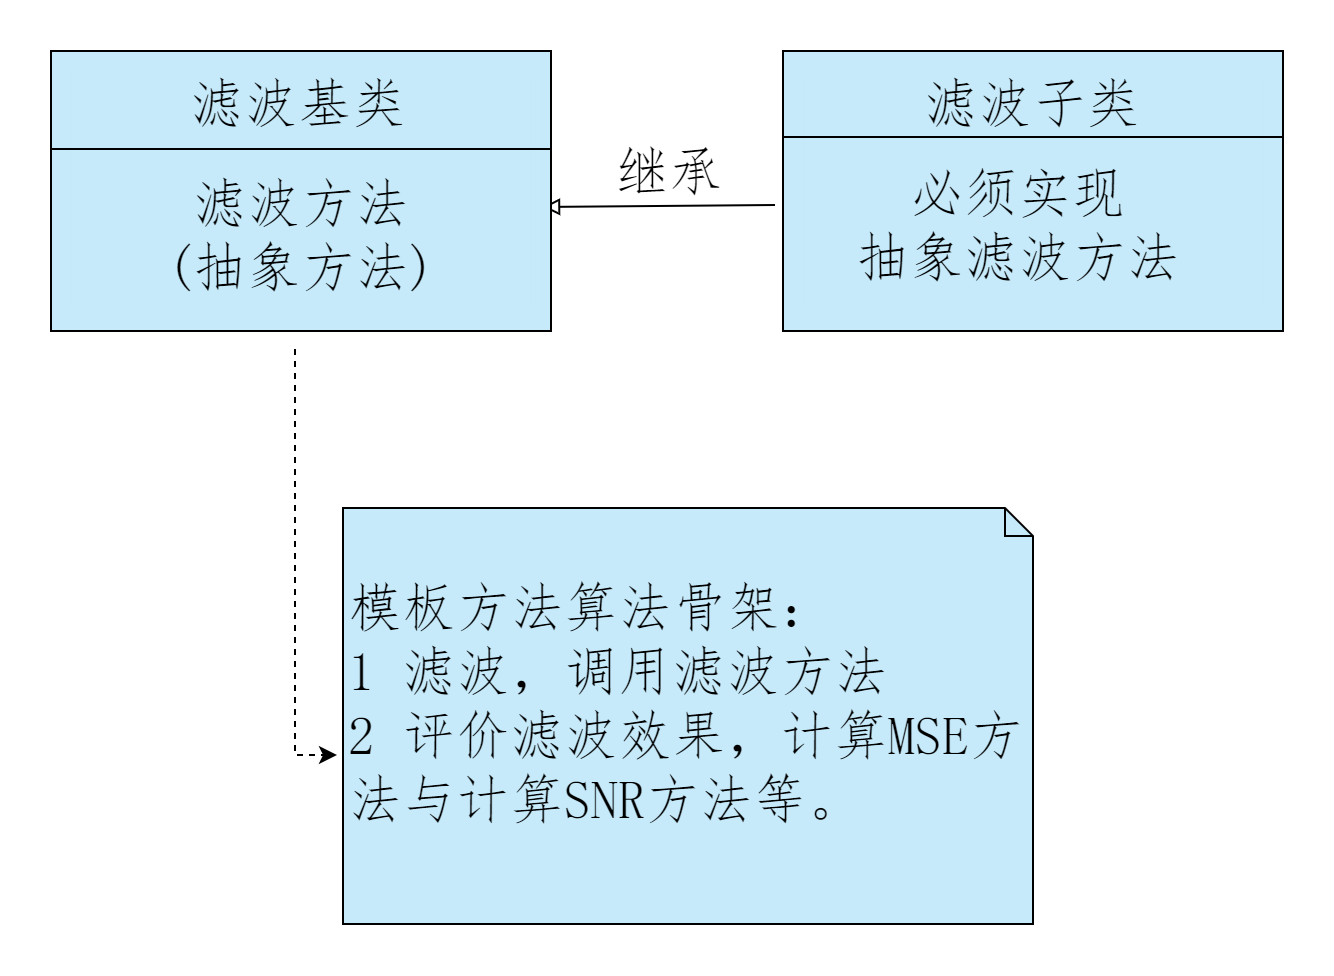
\includegraphics[width=.55\linewidth]{software/template}
    \caption{\label{fig:template2}滤波处理的设计}
\end{figure}

模板方法的基本原则是预定义一个操作中算法的骨架,而将延迟实现其中的关键步骤。
软件系统在数据读取过程所对应的抽象基类中定义了模板方法,并在模板方法中定义了数据读取过程的操作骨架。
基类中的读取方法被定义为抽象方法,真正的业务方法必须在基类的具体子类中实现。
当主程序需要进行滤波处理时,只需实例化特定子类后,在子类中调用上述模板方法。

与\autoref{fig:template}不同的是,在\autoref{fig:template2}中,滤波过程所对应的抽象基类中除定义了模板方法外,还定义了其他评价滤波效果的相关方法等。
而常用于评价滤波效果的均方误差与信噪比等指标可以设计为滤波基类的业务方法;而带通滤波器、小波滤波器等多种经典滤波算法可以在不同的滤波子类滤波方法中实现。

三、特征点定位与波形检测

本研究对PPG波形的检测过程进行了模式设计,
结合模板方法与工厂方法(Factory Method)\cite{Enrich2018},提出了一种基于初筛—复核—决策(screening-checking-deciding,SCD)的新型算法,其处理流程如\autoref{fig:detect2}所示。
由于特征点定位与波形检测的详细算法过程已经在第三章中详细介绍过,此处对其算法原理不再赘述。
\begin{figure}[htbp]
    \centering
    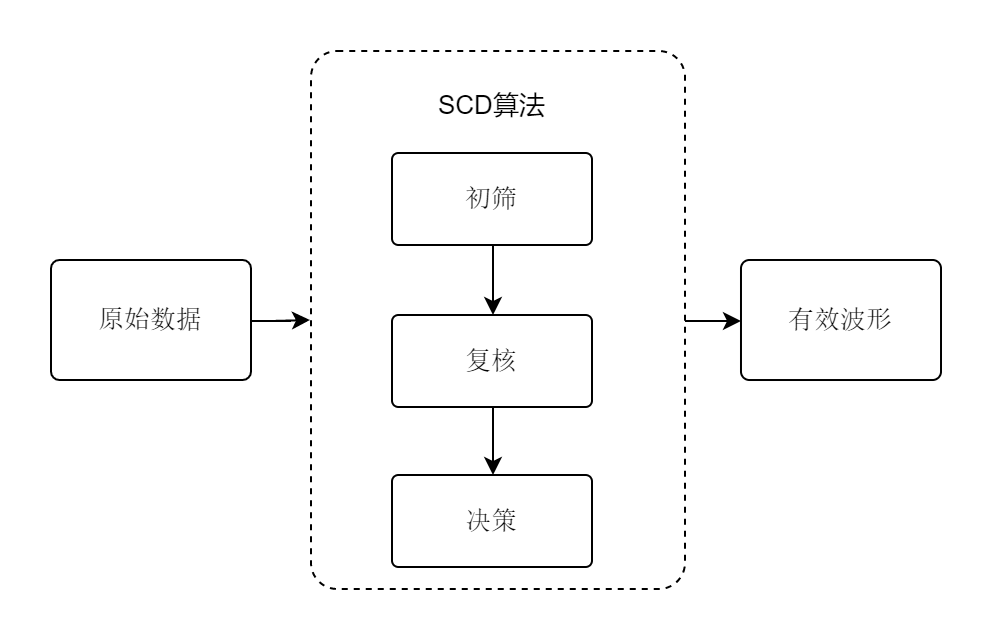
\includegraphics[width=0.65\linewidth]{software/scd}
    \caption{\label{fig:detect2}SCD算法检测流程示意图}
\end{figure}
\begin{figure}[htbp]
    \centering
    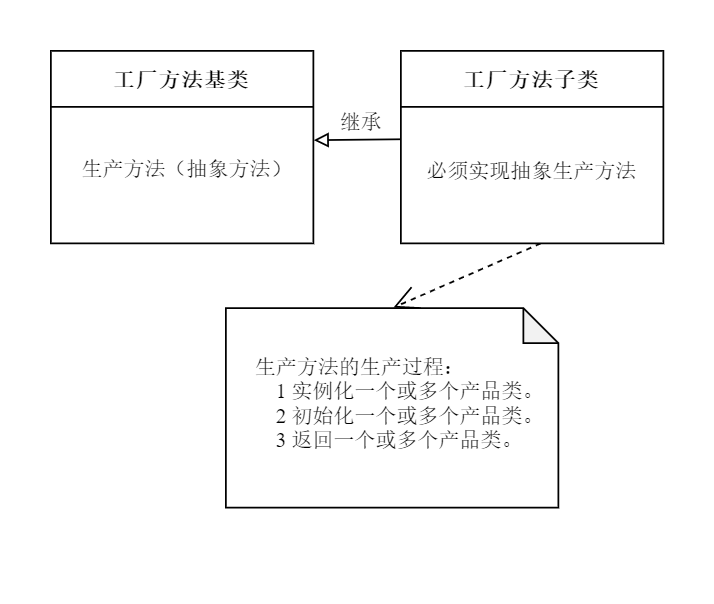
\includegraphics[width=.55\linewidth]{software/factory}
    \caption{\label{fig:factory}工厂方法的原理示意图}
\end{figure}

工厂方法的原则是定义一个用于创建对象的接口,让子类决定实例化具体的类。对\autoref{fig:detect2}中的SCD波形检测算法而言,
初筛、复核及决策阶段均按上述模板方法进行了设计,各阶段的具体业务方法均在对应的具体子类中得到实现。
在SCD算法运行时,这些子类并不是直接被实例化,而是作为特殊的“产品”,由一个额外的工厂类完成生产,如\autoref{fig:factory}所示。
该工厂类中定义了用于实例化、初始化这些产品的抽象生产方法,该抽象方法必须在工厂类的子类中实现。
若需设置或改变所需产品,只需在工厂类的不同子类中调整生产过程。
对SCD算法而言,在初筛及决策阶段对应的工厂类中,生产方法只返回一个产品对象;而在复核阶段对应的工厂类中,
生产方法则以列表的形式同时返回了多个产品对象。

四、特征计算

在第四章中,本论文定义了大量基于PPG形态学的特征参数。软件系统使用单例程模式(Singlon)对这些特征参数的计算过程进行了模式设计\cite{Li2015,Enrich2018},
这一过程如\autoref{fig:singleton}所示。

\begin{figure}[htbp]
    \centering
    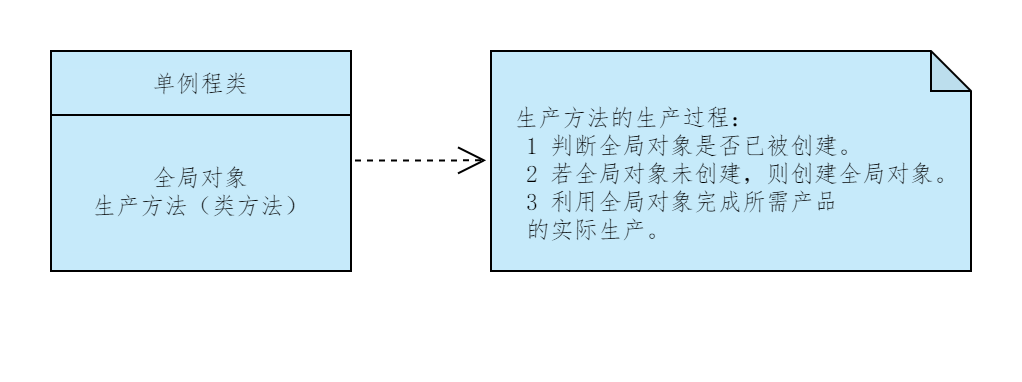
\includegraphics[width=.6\linewidth]{software/singleton}
    \caption{\label{fig:singleton}单例程模式的原理示意图}
\end{figure}

单例程模式的原则是保证一个类仅有一个实例,并提供一个访问它的全局访问点。
单例程模式在PPG形态特征计算模块得到了应用。由于PPG时域特征种类繁多,本研究在时域特征的抽象基类中定义了模板方法,
由模板方法负责调用特征的计算方法。计算方法在基类中被定义为抽象方法,也必须在具体的特征子类中实现。
而PPG时域特征的计算过程与其定义完全绑定,在处理不同PPG波形时创建不同特征实例是对内存资源的浪费。
因此,本研究使用单例程模式该过程进行了设计,单例程类自身不提供显式的构造方法,
此前所有可用特征的实例化过程被设计为单例程类的生产方法,且该方法只能作为类方法被调用。
在初次被调用时,生产方法会创建并保存单例程类本身的一个全局对象,并由全局对象完成生产返回所需产品;
此后的调用直接均由全局对象完成生产。单例程模式可以提升软件系统的工作效率、降低内存资源的消耗。

另外,预处理模块在时域特征的抽象基类额外定了两个属性$Order$与$Prefixes$。
这是因为某些特定的特征在计算时,可能需要一定的先导条件,需要预先计算好一定的先导特征。
因此,按照先导条件从无到有、从少到多、从简单到复杂的原则,在初始化特征时,给每个具体实现子类设置好其计算顺序
$Order$及保存着其先导特征$Order$的$Prefixes$,最后按照所有子类的计算次序$Order$遍历,即可保证所有特征均按指定顺序全部计算完毕。

五、数据导出

当对生理信号的预处理分析完成后,如何将分析处理结果进行保存是软件系统最后需要解决的问题。
导出的数据是以检测的PPG波形为基础,包含该波形所有形态特征。而在本研究中,多种新设计的特征参数往往是以向量的形式出现,
因此最后导出的结果将会大量出现波形——特征——向量(pulse-feature-vector)这种二级树状结构。
此外信号特征算法出现引入了新的信号特征、对已有特征值数值的保存形式进行更改等更迭将会直接引起数据存储格式的变化。
而常见的基于列表式的csv、txt等对这种树状数据格式的支持较差,需要借助新的数据储存格式来实现。

\begin{figure}[htbp]
    \centering
    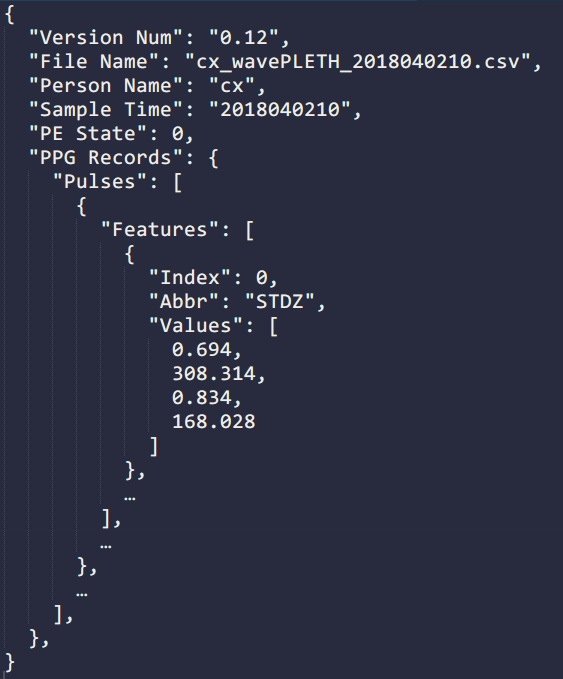
\includegraphics[width=\linewidth]{software/json}
    \caption{\label{fig:json}软件系统按JSON格式保存的数据示意图}
\end{figure}

扩展标记语言(Extensible Markup Language,XML) \cite{xml,Li2016}与JavaScript对象标记法(JavaScript Object Notation,JSON)\cite{json,Crockford2006}
是两种服务器端流行的数据交换格式。两者均可按照实际需求灵活定制存储规则,对较为复杂的数据结构
支持性好、拓展性强。但由于XML是基于标签描述数据的,在描述数组类型数据时,引入了大量冗余信息。
而JSON则对数组类数据有着更好的支持,有着更快的读写速度与更高的存储效率\cite{Nurseitov2009}。
因此,软件分析系统最终使用JSON作为数据交换格式,
而在具体实现时使用了中国阿里巴巴公司的开源JSON解析库fastjson\cite{fastjson}进行编码。
最后的导出数据如\autoref{fig:json}所示。在\autoref{fig:json}中,除基本数据特征外,与数据相关的文件信息及孕妇人口统计学信息也被保存至JSON文件。

六、多生理参数的兼容接口

尽管现阶段针对PE的研究主要基于PPG这种单一生理信号,但这并不排除以后的研究会引入更多人体生理信号进行分析的可能。
鉴于此,软件系统进一步设计了表征一般生理信号的抽象基类$AbstractBMESignal.class$,数据读取、预处理及信号特征计算过程均设计成抽象方法,
而PPG信号作为上述抽象生理信号的具体基类被设计为$Pulse.class$,而上文中介绍的具体处理过程均是对抽象基类中各抽象方法的实现。后续若有其他生理信号的分析需求,可以视情况
拓展实现心电$ECG.class$、脑电$EEG.class$等。由于这些子类都继承自$AbstractBMESignal.class$,因此可以确保这些子类具有相同的函数接口,方便将来可能的拓展。

\subsection{跨平台客户端模块}

在数据与处理模块的基础上,软件系统利用Java编程语言分别完成了PC客户端与Android客户端的设计开发。下面对其功能分别予以具体介绍。

一、PC客户端

软件系统借助VSCode在Windows系统下完成了PC客户端的开发。而由于Java本身的跨平台特性,该客户端也可方便在Linux等其他系统下进行编译运行。

1、功能与界面

PC客户端的交互界面如\autoref{fig:pc_ui}所示。\autoref{tab:pc_ui}对\autoref{fig:pc_ui}中软件界面的相关功能进行了进一步的说明。
其中,文件菜单选择对原始数据的打开及经分析后特征数据的导出;编辑菜单可以完成数据的预处理、分析等功能;
批处理菜单提供了大量数据进行处理分析的便捷操作方式;而帮助菜单则给出软件开发单位、软件版本号等信息。这些功能的进一步说明可参考\autoref{tab:pc_ui_menu}。
软件交互界面的波形显示区域可以展示当前打开数据文件的波形图,支持通过鼠标完成拖动、缩放等功能;对波形的波峰波谷等特征点的分析也在\autoref{fig:pc_ui}中有所标示。
与此同时,PC端软件也提供了较为丰富的右键菜单功能,提供了修改绘图颜色字体属性,支持选中当前波形直接复制至文件及连接打印机打印等功能。
由于这些右键功能意义明确,可直接通过菜单名理解,故不提供表格进行枚举解释。

\begin{figure}[h]
    \centering
    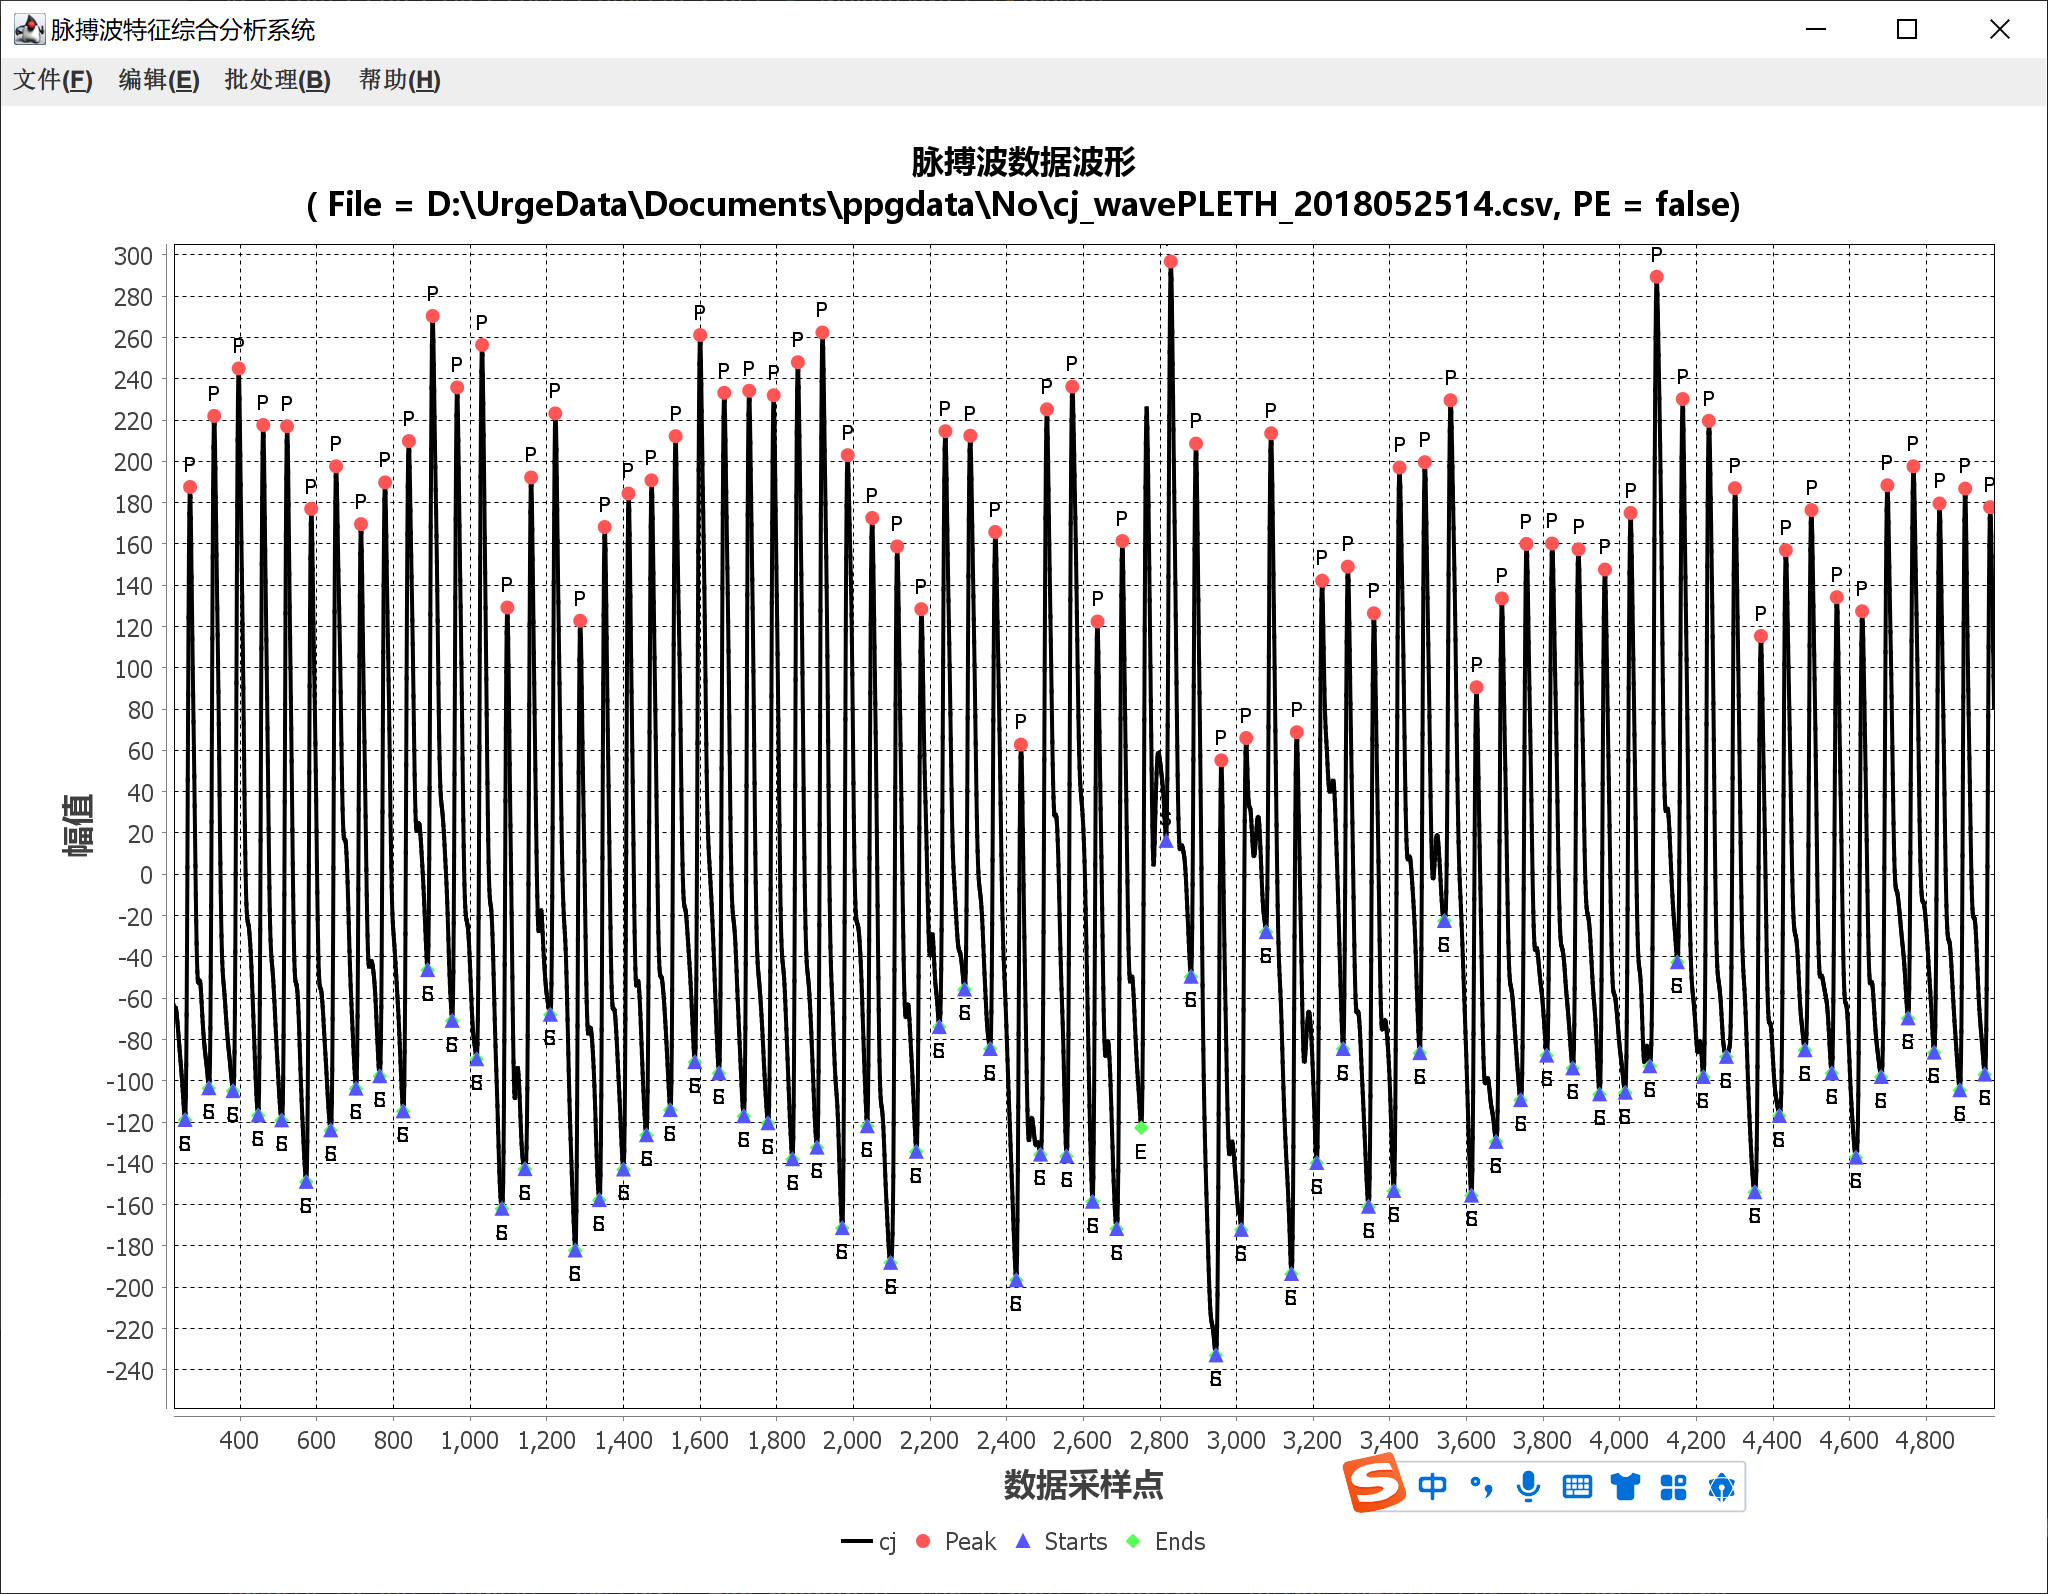
\includegraphics[width=\linewidth]{software/pc}
    \caption{\label{fig:pc_ui}PC端软件界面示意图}
\end{figure}

\begin{longtblr}
    [
        theme                   = {zju},
        caption                 = {PC端软件界面功能说明},
        label                   = {tab:pc_ui},
    ]
    {
        width                   = \linewidth,
        colspec                 = {X[1,c,m]X[3,c,m]X[1,c,m]X[3,c,m]},
        hline{1,Z}              = {\thickline},
        hline{2}                = {\thinline},
        rowhead                 = 1,
        row{odd}                = {bg=\oddcolor}, 
        row{even}               = {bg=\evencolor},
        row{1}                  = {font=\headfont,bg=\headcolor},
        row{2-Z}                = {font=\nonheadfont},
    }
    编号 & 功能 & 编号 & 功能 \\
    1 & 菜单栏 & 5 & 波形起点标记 \\
    2 & 文件路径及PE状态说明 & 6 & 波形终点标记 \\
    3 & 波形显示区域 & 7 & 右键功能菜单 \\
    4 & 波形峰值标记 & 8 & 图例 \\
\end{longtblr}

\begin{longtblr}
    [
        theme                   = {zju},
        caption                 = {PC端软件主菜单功能说明},
        label                   = {tab:pc_ui_menu},
    ]
    {
        width                   = \linewidth,
        colspec                 = {X[1,c,m]X[1.5,c,m]X[4,c,m]},
        hline{1,Z}              = {\thickline},
        hline{2}                = {\thinline},
        rowhead                 = 1,
        row{2-4,11-13}          = {bg=\oddcolor}, 
        row{5-10,14-15}         = {bg=\evencolor},
        row{1}                  = {font=\headfont,bg=\headcolor},
        row{2-Z}                = {font=\nonheadfont},
        cell{2}{1}              = {r=3,c=1}{c,m},
        cell{5}{1}              = {r=6,c=1}{c,m},
        cell{11}{1}             = {r=3,c=1}{c,m},
        cell{14}{1}             = {r=2,c=1}{c,m},
    }
    菜单 & 子菜单 & 功能说明 \\
    文件 & 打开 & 选择需要分析的PPG文件 \\
        & 上传单个文件 & 上传单个PPG文件的处理结果至云服务器\\
        & 上传目录下文件 & 上传目录下多个PPG文件的处理值云服务器端\\
    编辑 & 设置PE状态 & 标记当前PPG文件对应的孕妇的PE状态 \\
        & 波形校验 & 开启SCD算法自动校验波形 \\
        & 波形人工校验 & 启动人工校验波形功能\\
        & 导出检波结果 & 将检测到的PPG波形数据以Json形式保存至硬盘\\
        & 特征分析 & 开始计算检测PPG波形的特征参数 \\
        & 导出并上传 & 导出当前分析的所有分析结果,并将结果上传至云服务器 \\
    批处理 & 操作说明 & 显示批处理操作的帮助文档\\
        & 生成模板 & 选择要批处理分析的文件夹路径,并在目录下生成批处理模板\\
        & 开始批处理 & 选择经过人工调整确认过的批处理模版,开始批处理\\
    帮助 & 更新日志 & 显示软件的更新日志信息\\
        & 关于 & 显示软件的开发团队、版本信息等 \\
\end{longtblr}

2、处理流程与逻辑

PC端正常的处理流程如\autoref{fig:pc_process}所示。在选中需要分析的PPG文件后,软件系统会自动调用SCD算法的进行波形初筛,并将筛选结果在波形显示区域进行标注。
此时,点击波形检验菜单,SCD算法的检查与投票功能会被调用,会对此前的检验结果进行调整修整。用户可以通过鼠标放大观察整段数据的检测结果,若对
检测结果有异议,可以点击波形人工校验菜单进行校正。此时,用户可以选择导出波形的检测结果,将完整波形对应的数据段以及其相对原始数据的位置等信息导出。
随后,点击特征分析可以计算PPG波形的时域特征,点击导出并上传会将波形检测结果与特征计算结果以Json形式保存,同时这些数据也会被上传至云服务器进行后续分析。
\begin{figure}[htbp]
    \centering
    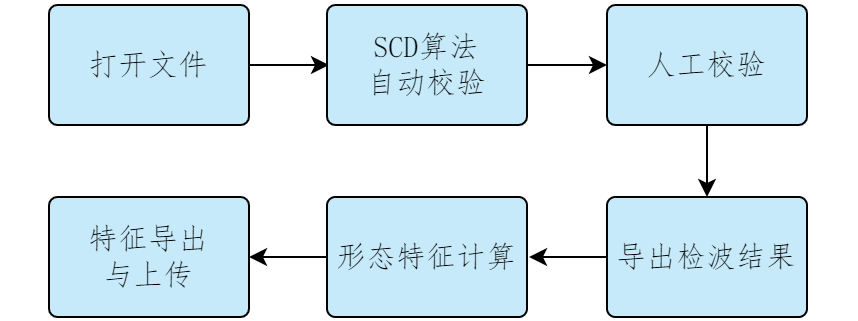
\includegraphics[width=.65\linewidth]{software/pc_process}
    \caption{\label{fig:pc_process}PC客户端程序的操作流程}
\end{figure}

除上述完整流程外,PC软件客户端也支持直接选择包含某次分析的生成结果的Json文件上传至云服务器和对指定目录下的指定PPG文件进行批量处理操作,这部分的详细介绍见下文。

3、特色功能说明

1)完善的日志记录

PC端软件借助Apache公司的log4j(log for Java)开源项目进行软件日志管理与输出,可将软件运行过程中的运行状态和中间变量等关键信息按级别
输出到不同日志文件中,方便系统开发与调试维护,如\autoref{fig:logs}所示。其中,日志输出级别包括OFF、FATAL、ERROR、WARN、INFO、DEBUG、ALL等,
其日志输出的重要性依次降低,但输出的详细程度递增。
\begin{figure}[htbp]
    \centering
    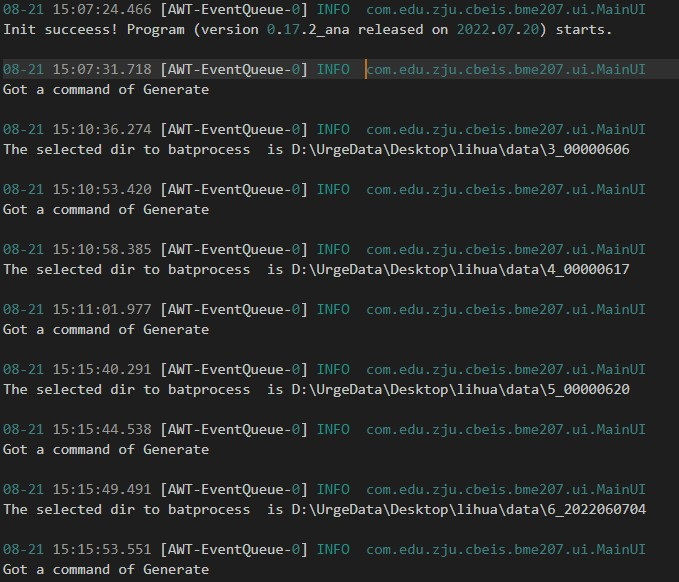
\includegraphics[width=0.8\linewidth]{software/logs}
    \caption{\label{fig:logs}PC客户端日志文件示意(局部)}
\end{figure}

2)人工校验波形

为解决SCD波形检测算法对某些极端数据的漏检、误检等问题,PC客户端还额外增加了对PPG波形的人工校验功能以精细控制PPG波形的增删,如\autoref{fig:manal_check}所示。

在\autoref{fig:manal_check}中,点击其中表格当前行末的跳转至按钮,软件界面会自动放大波形并跳转至当前选择波形,方便观察波形细节。
当需要删除已检波形时,只需在\autoref{fig:manal_check}中取消勾选波形行末的是否确认按钮;当需要调整波形起点、波峰及波谷时,只需双击相应数字单元格,
输入新的采样点序号近似值;当需要新增波形时,只需点击\autoref{fig:manal_check}中的增加新波形,并输入新的波形
的起点、波峰及波谷的近似采样点序号。点击校验当前行,PC软件会自动检查当前波形,并在起点、波峰及波谷的采样点序号的邻域内自动选择更为精确的数值,并将相应操作更新至
软件的波形显示区域;而点击校验所有行则会对所有波形进行相应的处理。
\begin{figure}[htbp]
    \centering
    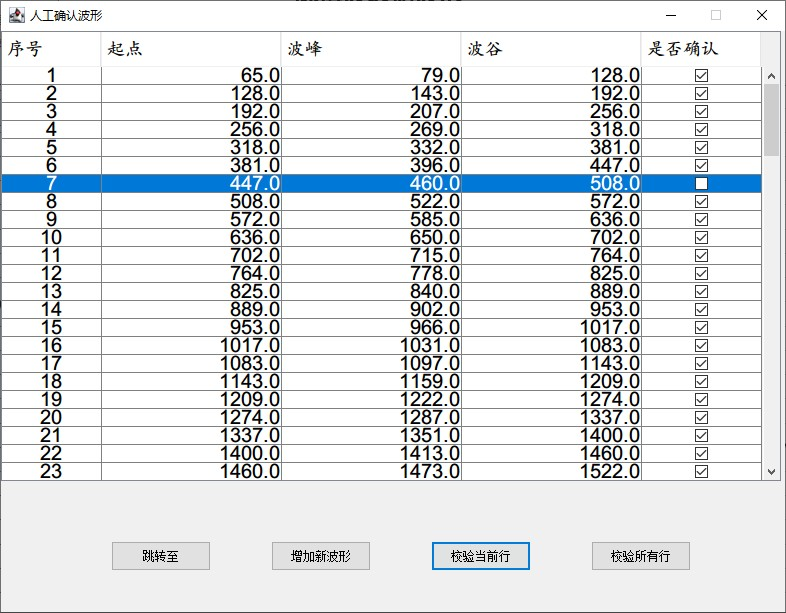
\includegraphics[width=0.8\linewidth]{software/manal_check}
    \caption{\label{fig:manal_check}PC客户端人工校验波形操作界面}
\end{figure}

3)批处理

在某些情景下,可能存在对已经分析过的PPG数据再次进行分析的情景,如PPG波形的特征算法得到更新、云服务器端的识别模型得到更新之后等。
则此时按上述处理逻辑与流程重新人工手动处理每一条原始PPG数据无疑显得耗时、低效且繁琐,特别是需要分析处理的数据量较大时。
为简化上述繁琐耗时的操作流程,PC客户端软件还额外开发了批量处理的功能。

\begin{figure}[htbp]
    \centering
    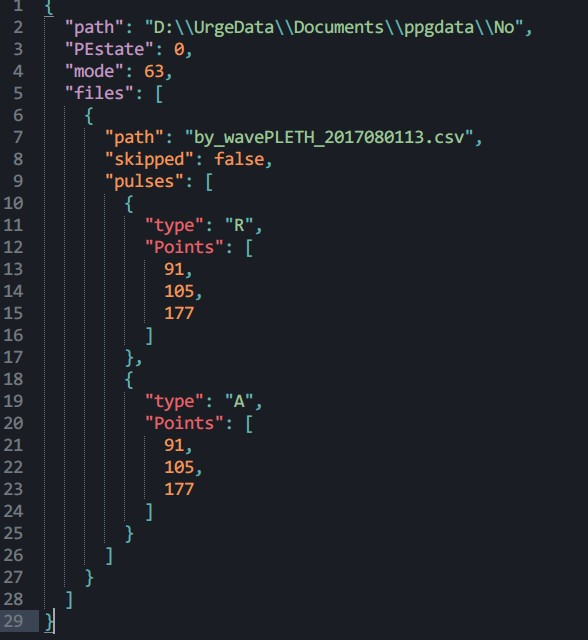
\includegraphics[width=0.7\linewidth]{software/configure}
    \caption{\label{fig:configure}PC客户端批处理配置文件示意}
\end{figure}

批量处理的核心思路是预先将多条PPG数据的处理过程中的各项人工操作写入配置文件中,随后按照该配置文件依次处理所有PPG数据原始记录文件。
具体操作时,需选择\autoref{fig:pc_ui}中的批处理菜单,再从如\autoref{tab:pc_ui_menu}所示的子菜单中选中生成模板。生成模板操作会要求选择一个
文件夹作为批处理的根目录,该根目录下所有的有效PPG原始文件会被记录,并在根目录下生成一个空白的配置文件模板。此时,需要用户
根据实际需要,自定义每一个PPG数据文件的个性化的处理流程,包括波形的计算与调整等。当批处理配置文件由用户更新完成后,最后可点击
从\autoref{tab:pc_ui_menu}所示的子菜单中选中开始批处理,选择打开该配置文件,等待PC客户端处理完成即可。
这一过程中的使用的配置文件范例如\autoref{fig:configure}所示,而\autoref{tab:configure}也对\autoref{fig:configure}中内容进行了进一步的解释与说明。

\begin{longtblr}
    [
        theme                   = {zju},
        caption                 = {PC客户端批处理配置文件配置项说明},
        label                   = {tab:configure},
    ]
    {
        width                   = \linewidth,
        colspec                 = {X[1,c,m]X[3,c,m]X[5,c,m]},
        hline{1,Z}              = {\thickline},
        hline{2}                = {\thinline},
        rowhead                 = 1,
        row{odd}                = {bg=\oddcolor}, 
        row{even}               = {bg=\evencolor},
        row{1}                  = {font=\headfont,bg=\headcolor},
        row{2-Z}                = {font=\nonheadfont},
    }
    配置项 & 意义 & 说明 \\
    path & 文件夹路径 & 选择路径后会自动生成,不建议修改\\
    PEstate & PE状态 & 0 为正常,1为PE,其他值无效 \\
    mode & 功能选择 & 有效区间为0-63,具体含义参见后文 \\
    files & 需要批处理的所有文件 & 选择路径后会自动生成,支持修改部分配置项 \\
    files下的path & 需要处理的PPG文件名 & 选择路径后会自动生成,不建议修改\\
    skipped & 是否跳过处理该文件 & true跳过,false不跳过,默认不跳过\\
    pulses & 需要调整的PPG波形 & 默认为空,需要自定义修改 \\
    type & PPG波形调整类型 & R为移除,A为新增,其他值无效\\
    Points & PPG波形特征点坐标 & {需要波形起点、波峰、波谷等三个数值。\\可以不精确,可自动在邻域内精确调整}\\
\end{longtblr}

\autoref{fig:configure}所示的配置文件本质上仍是一个Json文件,其中的大部分配置项的具体含义及可选数值范围已经在\autoref{tab:configure}进行了说明。
对于\autoref{fig:configure}中的mode配置而言,其数值确定了所需要进行的批处理操作。
目前mode支持\autoref{tab:pc_ui_menu}中波形校验、波形人工校验、导出检波结果、特征分析、导出并上传等6种操作,
这些操作分别通过mode的1位来完成控制,其中波形校验对应mode的最低位。mode的默认值为31,即$0b011111$,即对当前文件进行除数据特征上传外的所有操作。
需要注意的是,尽管mode的可选值域是0-63,但由于可配置的6个操作有着逻辑上的依赖关系,某些配置可能会导致程序无法运行。
因此,\autoref{fig:configure}所示的配置文件可对\path{D:/UrgeData/Documents/ppgdata/No}文件夹下的\path{by_wavePLETH_2017080113.csv}等文件进行批处理。其中,PEstate被设置为0,表示当前目录下全为健康人群数据文件。
mode被配置为63,所有文件会完成全部6项批处理操作。而在对\path{by_wavePLETH_2017080113.csv}文件处理时,
不需跳过该文件,对算法的自动检测结果需先移除$(91,105,177)$处的PPG波形,再在$(91,105,177)$处新增一个PPG波形。

二、Android客户端

软件系统借助Android Studio在Windows系统下完成了Android客户端的开发,并在中国小米公司生产的Redmi Pad SE上测试通过。
其中,Redmi Pad SE的Linux内核版本为5.10.101,Android版本为12。

1、功能与界面

\autoref{fig:android_ui}展示了软件分析系统在Redmi Pad SE上运行效果。为充分利用Pad显示界面,菜单栏默认隐藏,需要使用时可点击按钮唤出。
\begin{figure}[htbp]
    \centering
    \subfigure[默认界面]{
    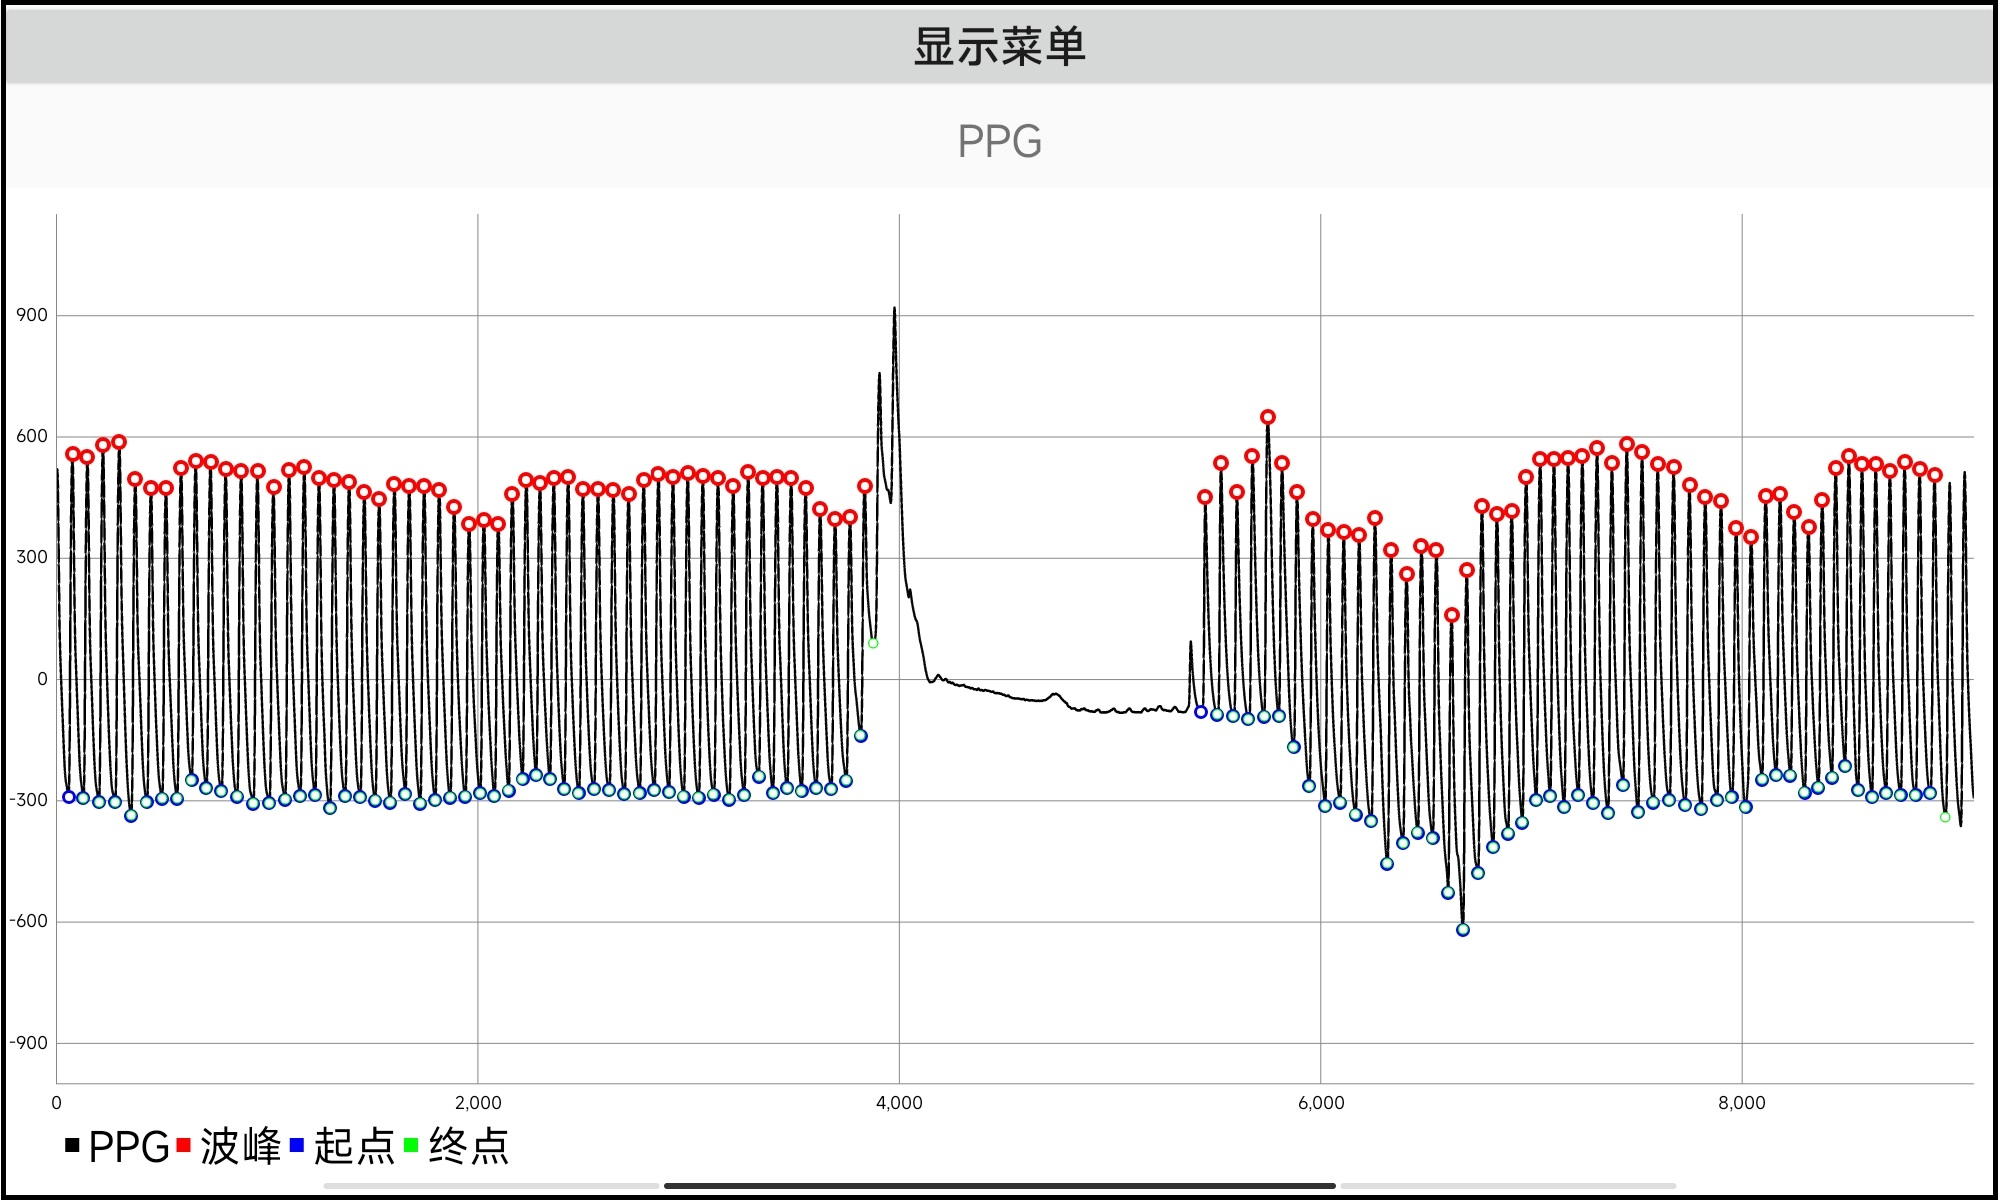
\includegraphics[width=11cm]{software/android}
    }
    \quad
    \subfigure[菜单唤出界面]{
    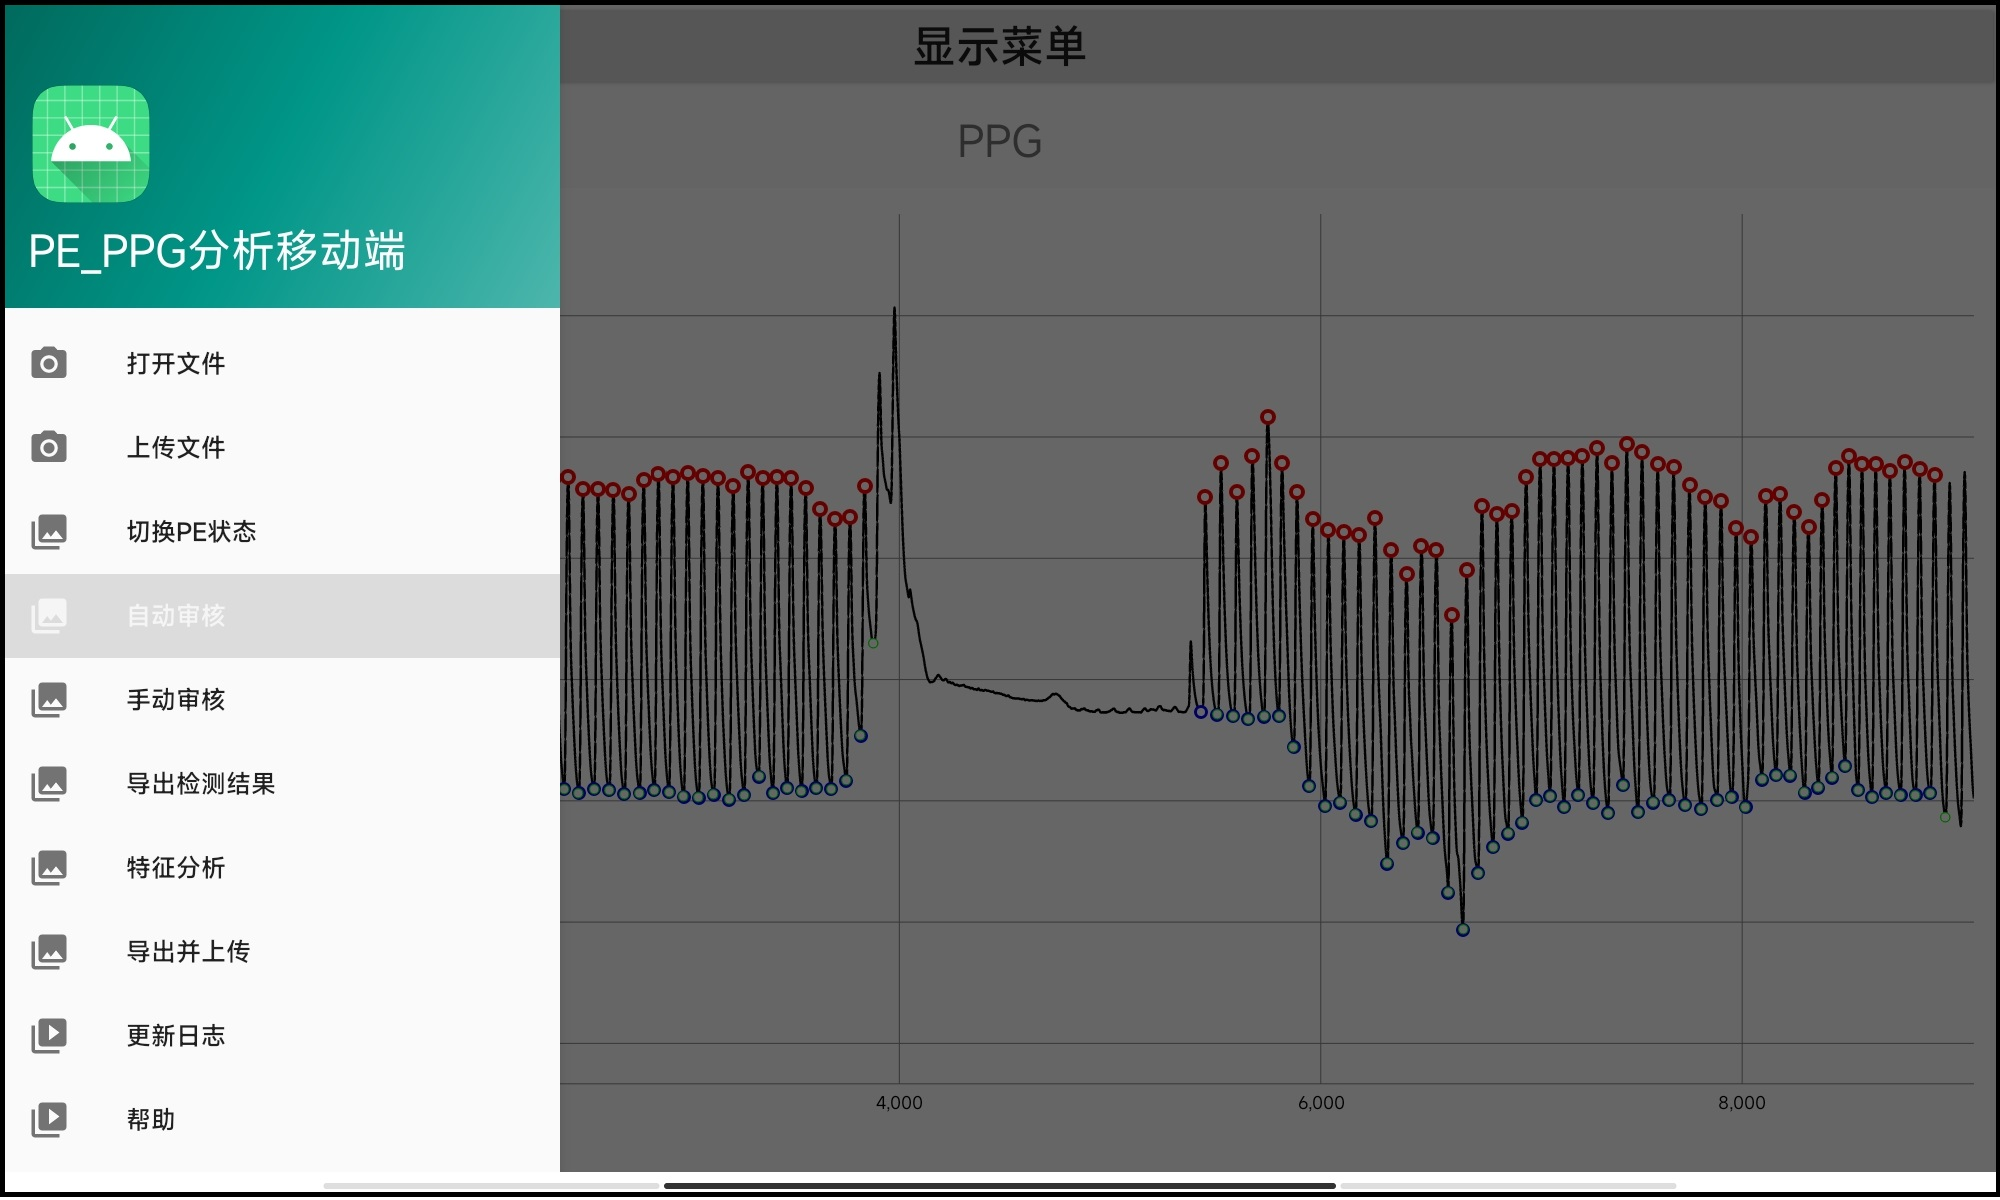
\includegraphics[width=11cm]{software/android_menu}
    }
    \caption{\label{fig:android_ui}Android客户端运行界面}
\end{figure}

另一方面,考虑到Android客户端的实际使用场景,上文介绍的PC客户端特色功能目前未在Android客户端下实现。
但除此之外,Android客户端与PC客户端整体功能相近、操作类似,故在此处不再进行相关赘述。

2、组件区别

由于Android系统独立于Java社区,主要由美国Google公司负责维护及更新,因此经常会出现某些Java组件在PC端与Android端的生命周期不一致的现象。
这也导致部分PC端可用的Java组件在新版本的Android系统下不被支持。因此,软件系统的特定功能需要针对具体操作系统平台选取恰当的组件完成功能开发。
图\autoref{tab:platform}展示了PC端与Android移动端相同软件功能在具体实现组件上的差异。

\begin{longtblr}
    [
        theme                   = {zju},
        caption                 = {PC端与Android移动端部分软件开发组件对比},
        label                   = {tab:platform},
    ]
    {
        width                   = \linewidth,
        colspec                 = {X[1,c,m]X[1,c,m]X[1,c,m]},
        hline{1,Z}              = {\thickline},
        hline{2}                = {\thinline},
        rowhead                 = 1,
        row{odd}                = {bg=\oddcolor}, 
        row{even}               = {bg=\evencolor},
        row{1}                  = {font=\headfont,bg=\headcolor},
        row{2-Z}                = {font=\nonheadfont},
    }
    功能特征&PC&Android\\
    数据上传&HttpClient\cite{HttpClient}&Retrofit\cite{Retrofit}\\
    数据图表显示&JFreeChart\cite{JFreeChart}&MPAndroidChart\cite{MPAndroidChart}\\
\end{longtblr}

\subsection{PE识别模型训练生成模块}
PE识别模型训练生成模块是软件系统的核心,基于已经提取好的数据特征完成识别模型的训练生成任务。在对训练好的PE分类识别模型进行评估后,
综合性能表现好的识别模型才会被部署至云服务端,供PC客户端与Android客户端调用,以识别预测新数据。而由于Python在机器学习领域的广泛普及应用,
此模块的所有编程设计与实现全部基于Python完成,以下为具体介绍。

一、数据合并

如前文所述,软件系统的客户端程序最终会把检测得到PPG波形数据与PPG时域特征分别以Json文件的形式保存至本地并上传至云服务器。而前文中已经介绍过,
Json文件的构成更符合一棵数据“树”的概念。为从多棵这样的数据树中构建出完整的特征数据集矩阵,显然需要一个数据合并的过程。
这也即第四章中提及的的脉搏波多维度时域特征集(photoplethysmographic multidimensional
time-domain feature set,PPGMTFS)与脉搏波采样序列时域特征集(photoplethysmographic sampling series time-domain feature set,PPGSSTFS)的生成过程。
\begin{figure}[htbp]
    \centering
    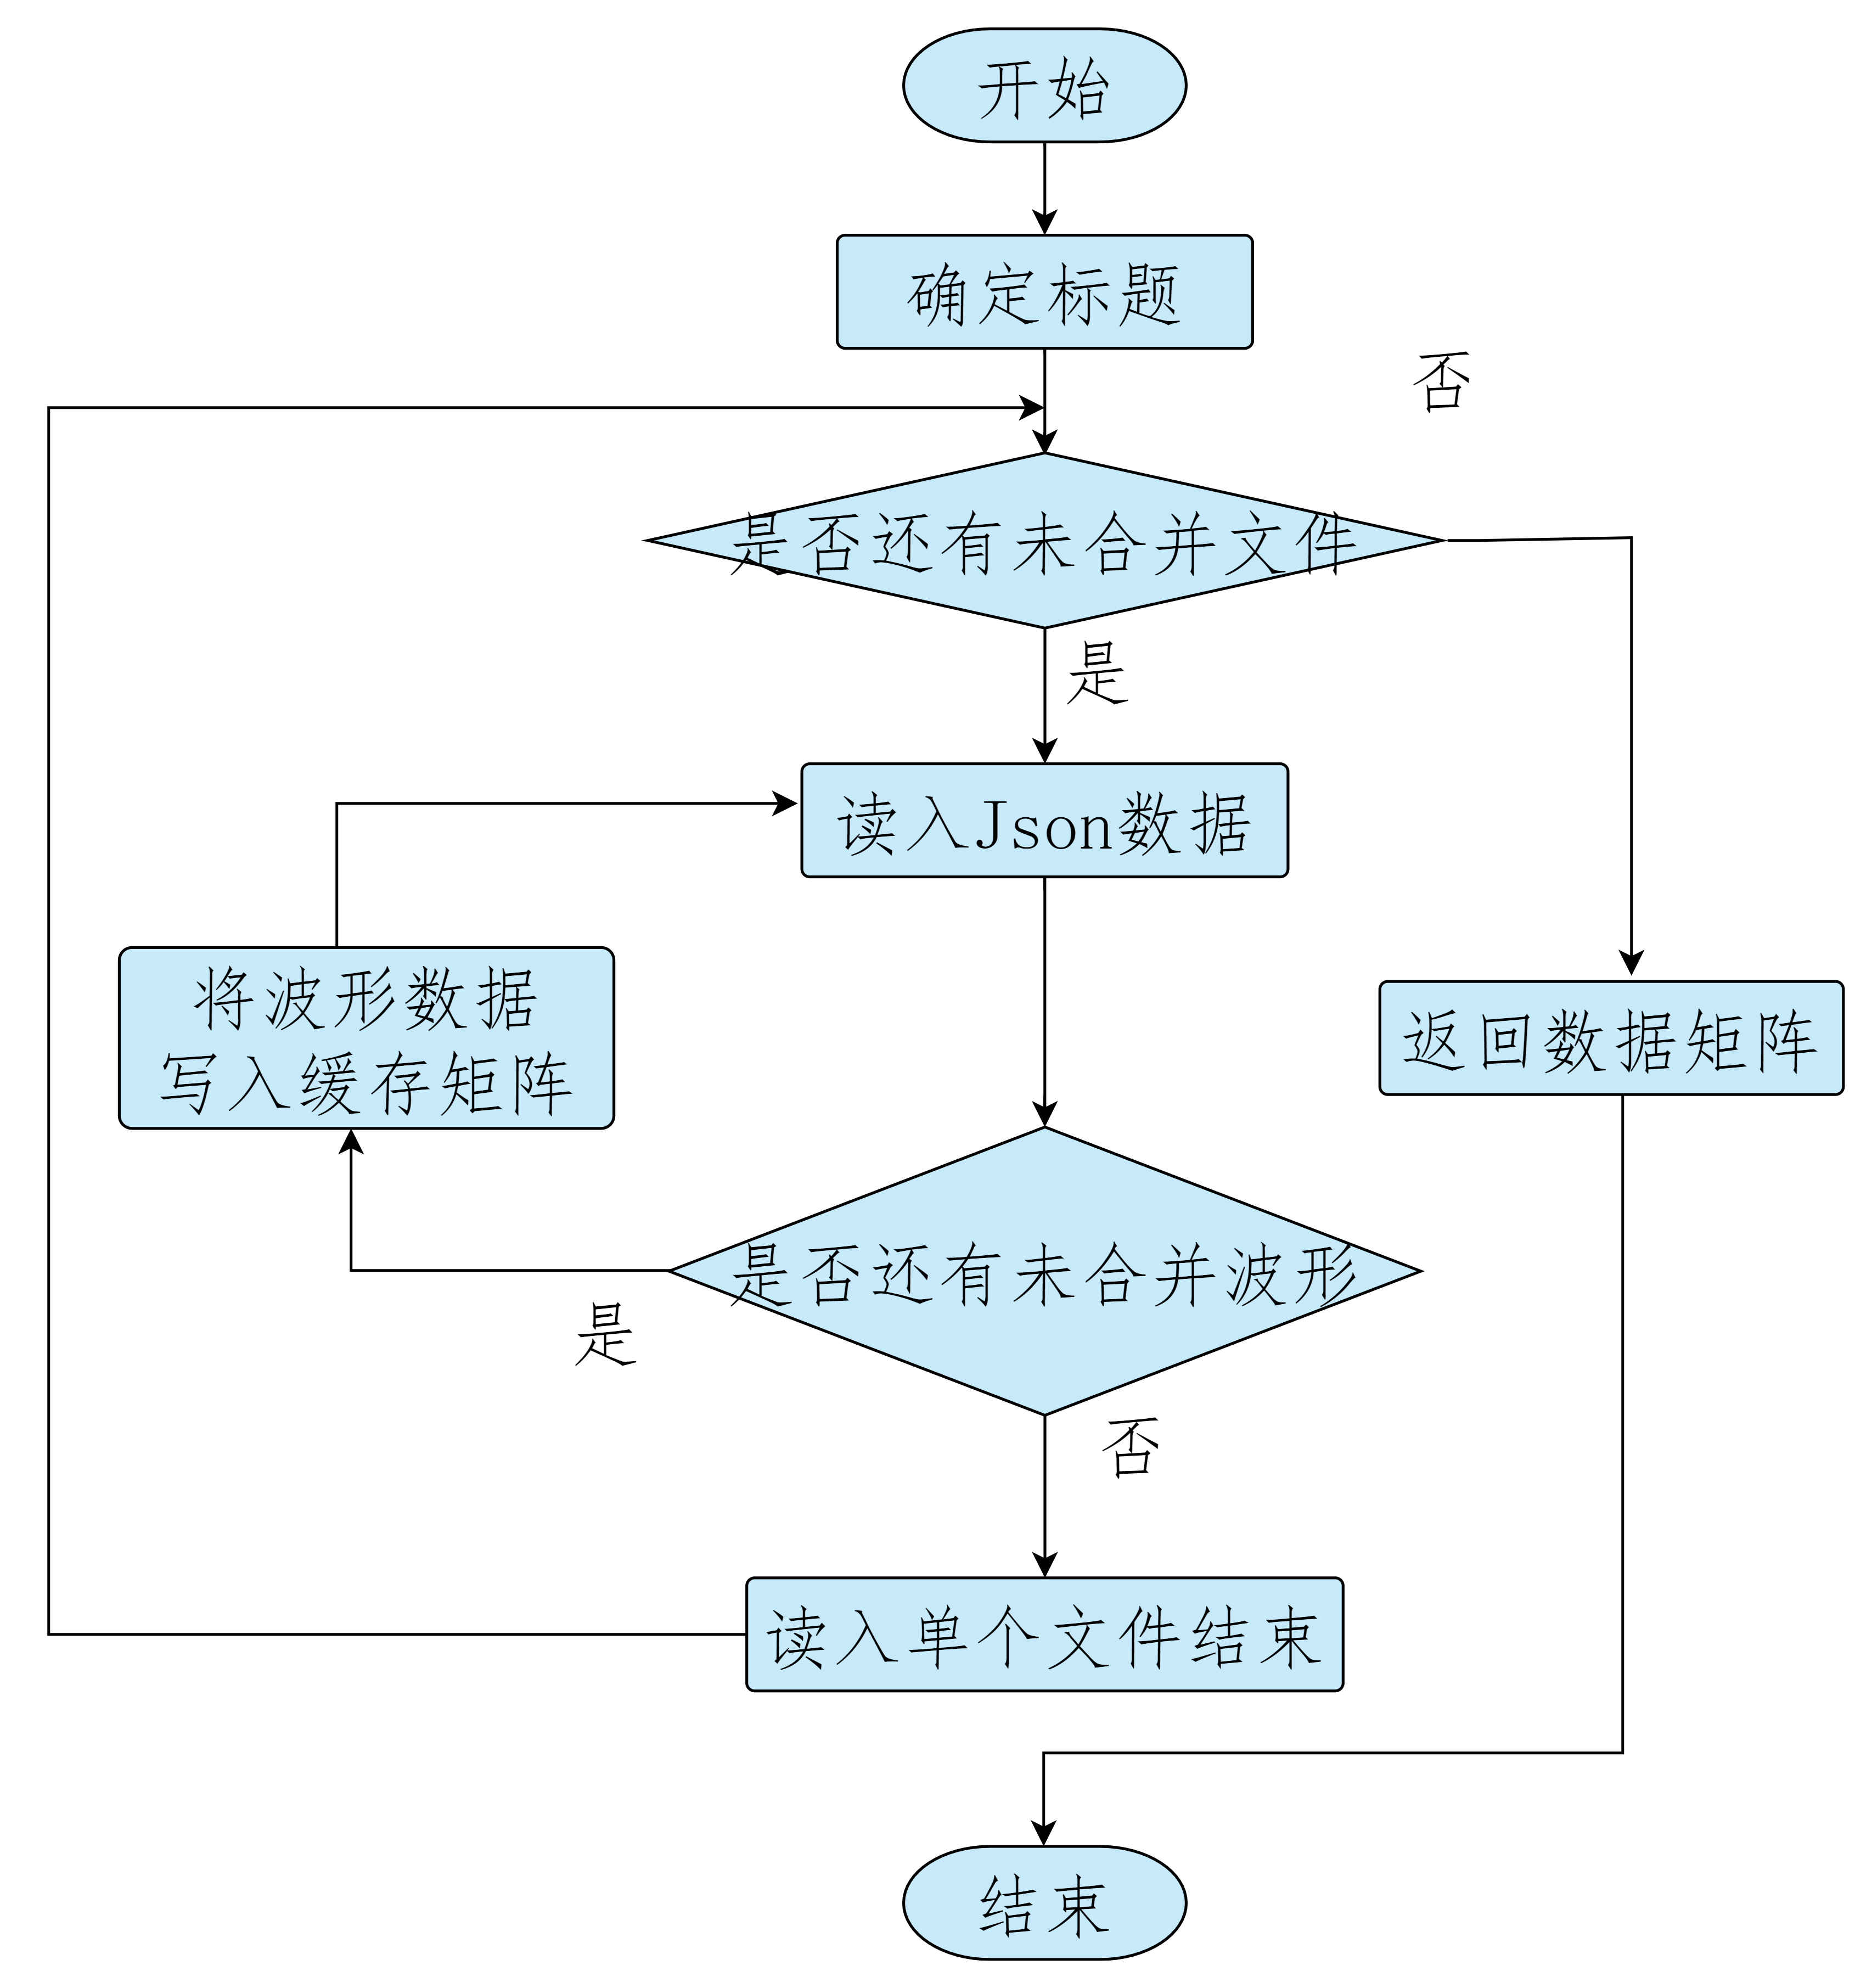
\includegraphics[width=.65\linewidth]{software/mergedata}
    \caption{\label{fig:mergedata}数据合并流程图}
\end{figure}

模块对数据合并的处理流程如\autoref{fig:mergedata}所示。依次读取需要合并的数据特征文件,确定生成矩阵的标题栏,记录下包括软件版本号、原始PPG数据文件名、数据患者名、PE状态等基本信息,
随后开始记录数据特征文件的所有特征数值,为了后续分析方便,PPG波形序号也被同时记录。而当生成PPGSSTFS时,需要根据PPG波形对齐策略的选择,将原始采样值量化至指定区间内。
按此方式依次处理完所有文件即可得到最终的数据集矩阵,而考虑到数据格式的兼容性的需要,数据集矩阵最终会以csv格式进行保存。

二、数据划分

如第四章介绍过的,为使后续经由不同机器学习算法训练所得的PE识别模型的性能具有可比性,需要通过控制变量法,让所有的机器学习模型在相同的训练数据集上训练模型,并在相同测试
数据集上评估性能。
\begin{figure}[htbp]
    \centering
    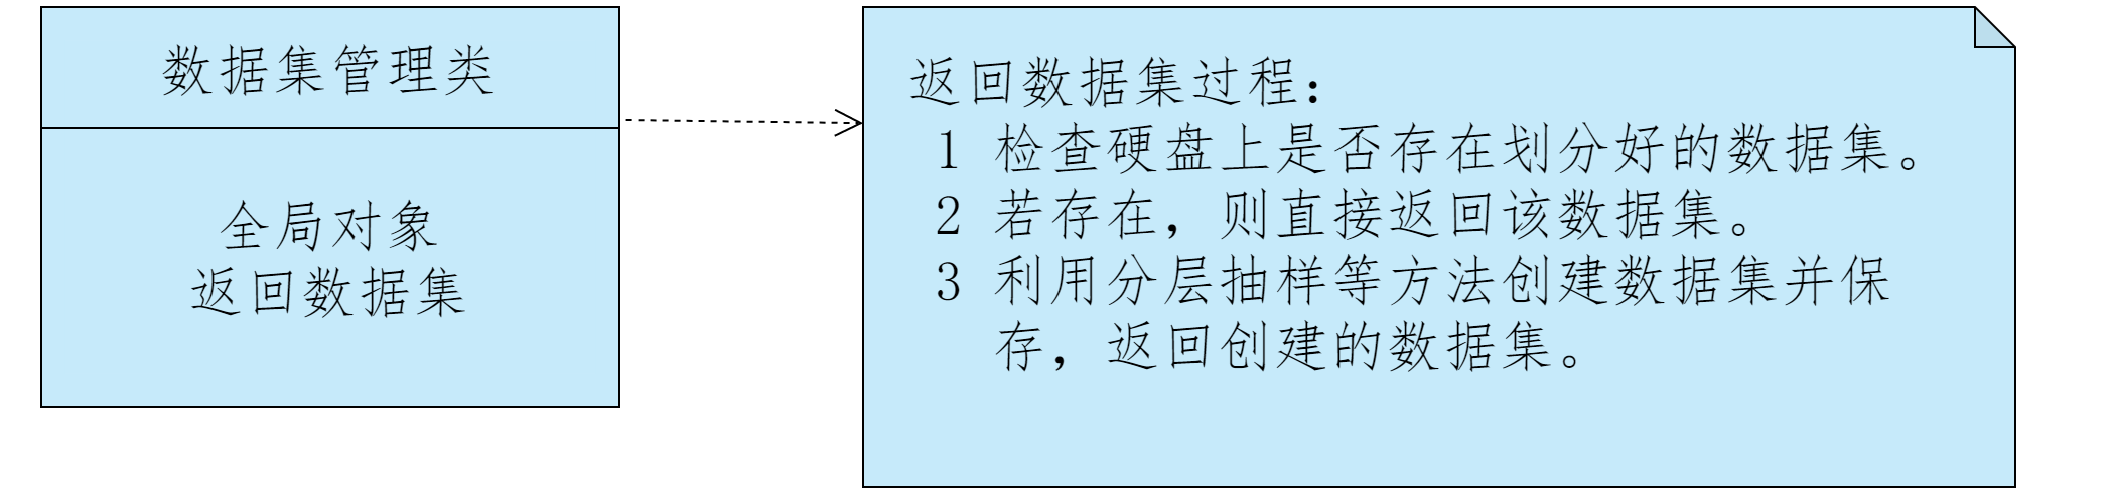
\includegraphics[width=.65\linewidth]{software/loaddataset}
    \caption{\label{fig:loaddataset}数据集划分创建过程示意图}
\end{figure}

本模块对数据划分的流程如\autoref{fig:loaddataset}所示。一个单独的数据集管理类负责返回所有模型训练、评估的训练集与测试集,而在该类内部,需要返回数据时,函数都会先去检查硬盘上是否已有划分好的数据集。
如果存在这样的数据集,则直接读取硬盘上数据集并返回;否则,函数会调用数据集分层抽样等函数并生成特定的数据集,将该数据集保存至硬盘上后返回该数据集。
而对比数据预处理模块的特征计算的\autoref{fig:singleton}可以发现,上述介绍的数据划分方式也可以视为一种广义上的单例程模式,区别在于后者多了一次对硬盘数据的检查和读取。

三、模型训练与保存

软件系统所有的PE识别模型均是借助Python下Sklearn工具包完成的。而单个PE识别模型的具体构建过程通常涉及载入数据、在训练集上进行训练、考察训练集上的性能、在
测试集上测试等等操作,且其中的某些步骤往往涉及到多个参数的计算与比较。当需要评估对比的机器模型过多时,这一些列的操作会给编程带来麻烦,且极易疏漏。
另一方面,由于Python本身是一种动态类型的编程语言,强调在运行时确定对象的类型,而非在编译时确定其类型。这意味着Python不会检测变量的具体类型,而是关注变量
是否具有特定的属性与方法。而Sklearn本身在设计过程中均遵循了统一规范,不同的机器学习算法均提供了相同的API函数。因此,软件系统在此基础上对不同机器学习算法进行了一层封装。

在本软件系统中,MyClasssifer是封装之后的类名,可直接用Sklearn工具包中的具体分类算法的实例初始化该类。除此之外,该类只有四个公共函数接口,
第一个为设定MyClasssifer所使用的分类算法的实例的初始化函数$init()$,该函数要求初始实例必须为Sklearn工具包中有效算法实例;
第二个为设定模型训练所需的训练集与测试集数据函数$load\_data()$;第三个为开始训练并评估的$fit\_predict()$函数,该函数封装了机器学习算法在训练集与测试集上的全部处理操作过程;
最后一个为对模型进行超参数网格搜索的函数$grid\_search()$。特别地,在$fit\_predict()$函数中集成封装了Sklearn工具包中各算法模型的多项重要函数,其处理流程如\autoref{fig:fit_predict}所示。
综上,借助封装后MyClasssifer类,评估不同的机器学习方法在同一批数据集上的表现的过程将得到进一步地简化,在实现代码的最小化的同时,也避免了算法模型训练过程的代码遗漏等问题,从而简化了模型训练过程。

\begin{figure}[h]
    \centering
    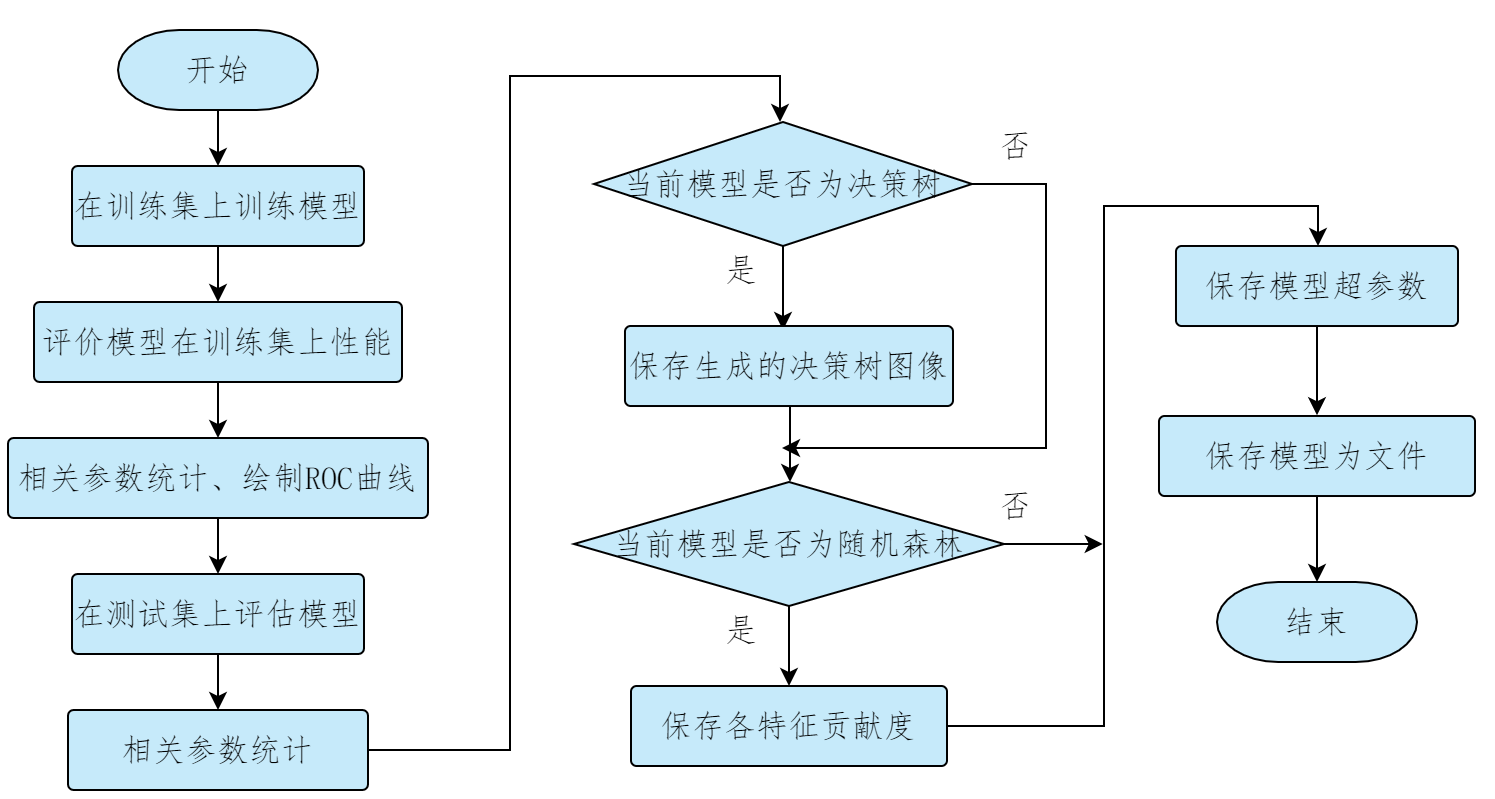
\includegraphics[width=.38\linewidth]{software/fit_predict}
    \caption{\label{fig:fit_predict}封装后的$fit\_predict()$函数处理流程图}
\end{figure}

注意在\autoref{fig:fit_predict}中,为使训练好的机器学习模型供后续上传至云服务器使用,MyClasssifer的$fit\_predict()$函数也将生成的最终模型与训练模型的超参数进行了保存。
除以随机森林为代表的部分随机性强的机器学习算法外,保存模型生成的超参数可确保只要给定相同的数据集,使用相同的算法在相同的超参数的条件下,就可以复现出完全相同的机器学习模型。

四、日志记录

与此前的客户端程序类似,为方便调试与记录模型训练模块在训练生成PE识别模型过程中的各项参数与中间变量等信息,模型训练模块也开发了程序日志记录功能。
而这一功能的开发基于Python下的logging包。

日志记录logging包中也支持设置日志等级,可在不同的版本(如开发环境、生产环境)上通过设置不同的输出等级来记录对应的日志,非常灵活。
其中,日志输出级别包括DEBUG、INFO、NOTICE、WARNING、ERROR、CRITICAL、ALERT、EMERGENCY等。而在具体使用logging包时需要通过一个Json文件进行
相关功能的配置,具体配置过程可参见logging包官方文档,这里不再赘述。\autoref{fig:clflog}给出了模型训练生成模型最终的日志记录示意。
\begin{figure}[htbp]
    \centering
    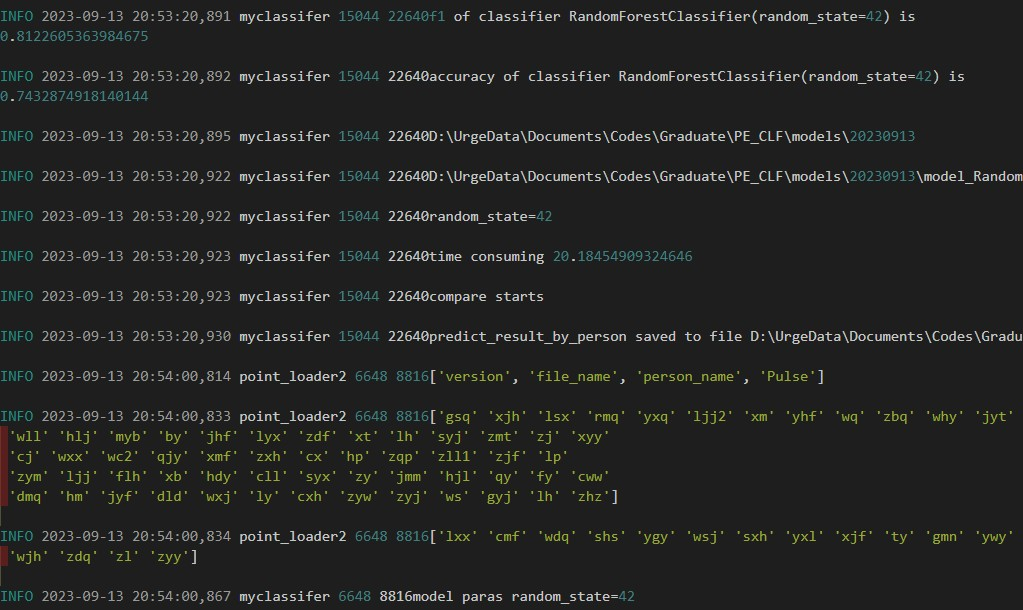
\includegraphics[width=.8\linewidth]{software/clflog}
    \caption{\label{fig:clflog}PE识别模型训练模块的日志记录示意}
\end{figure}

\subsection{云服务器模块}
云服务器模块在某种意义上可以看作为客户端软件与PE识别模型训练生成模块的中间件。云服务器端接收来自客户端的特征数据,在一定的校验确认数据无误后,
根据客户端具体请求内容,选择一个或多个已经训练好的机器学习模型进行新数据的识别预测,并将结果返回至客户端。为方便后续可能的二次开发,所有客户端的
发送来的原始数据都会被保存至数据库中。

需要注意的是,云服务器模块在设计时是可以直接使用第三方商业公司提供的具有公网IP地址的云服务器等业务。但在本软件系统的研发过程中,出于方便开发的角度,暂时仅使用了
局域网进行环境搭建模拟与后续测试。以下为云服务器模块的具体介绍。

一、网络协议选择与数据接口设计

为使客户端软件与云服务器端能够进行数据通信与数据交换,显然需要借助一定的网络协议。本软件系统最终选择了最为常见的超文本传输协议(Hypertext Transfer Protocol,HTTP)进行
两者间的数据通信。HTTP是一种简单的请求——响应协议,它通常运行在TCP之上,同时,HTTP也指定了客户端可能发送给服务器的消息类型以及能得到何种响应。

1、POST与GET

HTTP协议中定义了很多与服务器的交互的方法,而PUT、DELETE、POST与GET则是其中最基本的四种。一般而言,一个URL地址描述了一个互联网上的资源,而HTTP协议中的
PUT、DELETE、POST与GET等方法则对应着对这个资源的增、删、改、查等基本操作。其中,GET方法与POST方法最为常见,在互联网应用中使用的最为广泛。
GET方法与POST方法均能向服务器端传递数据,但两者之间也存在着一定的差异,如\autoref{tab:get_post}所示。

\begin{longtblr}
    [
        theme                   = {zju},
        caption                 = {GET方法与POST方法对比},
        label                   = {tab:get_post},
    ]
    {
        width                   = \linewidth,
        colspec                 = {X[1,c,m]X[3,c,m]X[3,c,m]},
        hline{1,Z}              = {\thickline},
        hline{2}                = {\thinline},
        rowhead                 = 1,
        row{odd}                = {bg=\oddcolor}, 
        row{even}               = {bg=\evencolor},
        row{1}                  = {font=\headfont,bg=\headcolor},
        row{2-Z}                = {font=\nonheadfont},
    }
    &GET&POST\\
    常用场景&获取、查询信息&更新资源信息\\
    数据传递方式&请求参数与数值附加在URL后&封装在HTTP请求中\\
    传递数据量&受限,一般为1024个字符&无限制\\
    编码方式&只允许ASCII字符&没有限制,也允许二进制数据\\
    安全性&较差,数据是URL的一部分&较安全,参数不会被记录保存\\

\end{longtblr}

鉴于\autoref{tab:get_post}所示,POST方法较GET方法功能更为强大,能够同时传递文本数据与二进制文件数据,因而被选为软件系统的客户端与云服务器端的通讯方式。

2、POST方法的参数设计

客户端在将需要上传的参数、数据进行POST封装时,所有的数据都会以键值对的形式进行映射。而为了方便服务器端的解析,将数据的键是否以“file”结尾作为区分文件数据与文本数据的标志,
并据此选择将与键对应的值以文件形式封装或文本形式封装,这一过程如所示。而服务器端在接受到POST请求后,在解析时数据时,会首先检查数据的键是否以“file”结尾,随后
选择对应的解析处理方式。截止目前,客户端程序通过POST方法向云服务器端提交数据的通讯过程中涉及到的所有参数如\autoref{tab:post_paras}所示,其中文件类数据在表格中用粉红色底色
进行了突出显示。
\begin{longtblr}
    [
        theme                   = {zju},
        caption                 = {客户端在POST方法中上传的所有参数},
        label                   = {tab:post_paras},
    ]
    {
        width                   = \linewidth,
        colspec                 = {X[1.5,c,m]X[3,c,m]X[1,c,m]X[1,c,m]X[2.5,c,m]},
        hline{1,Z}              = {\thickline},
        hline{2}                = {\thinline},
        rowhead                 = 1,
        row{odd}                = {bg=\oddcolor}, 
        row{even}               = {bg=\evencolor},
        row{1}                  = {font=\headfont,bg=\headcolor},
        row{2-Z}                = {font=\nonheadfont},
        cell{10,11,12}{3,4}     = {bg=\emphacolor},
    }
    参数的键名&参数值的含义&{数据流\\类型}&数据类型&备注\\
    project&上传的数据归属的具体项目&文本&字符串&{值固定为PE,代表数据隶属本论文基于PE的研究}\\
    data\_type&上传的数据所属生理信号类别&文本&字符串&{值固定为PPG}\\
    client&上传数据的客户端类型&文本&字符串&值为PC或Android\\
    version&上传数据的客户端程序版本号&文本&字符串&不同客户端软件版本号可能不同\\
    algorithm\_version&数据预处理模块的算法版本号&文本&字符串&不同客户端算法版本可能不同\\
    person&上传数据对应的孕妇名&文本&字符串&{遵循医学伦理学相关标准,省略孕妇具体姓名,仅以拼音缩写代替}\\
    pe\_state&上传数据对应孕妇的PE状态&文本&整型&0为健康孕妇,1为PE患者,2为待定\\
    source&此次上传对应的原始PPG文件名&文本&字符串&\\
    source\_file&此次上传对应的原始PPG文件数据&文件&文件数据&按二进制编码成数据流发送\\
    feature\_file&基于原始PPG数据计算得到的特征数据&文件&文件数据&按二进制编码成数据流发送\\
    point\_file&基于原始PPG数据计算得到的波形采样值数据&文件&文件数据&按二进制编码成数据流发送\\
    sample\_time&原始数据的采集时间&文本&字符串&{可选项,本论文中由于导出数据包含数据采样时间,故增设该值}\\
    predict&本次上传的数据是否需要进行预测分析&文本&字符串&值为True或False\\
    model&本次上传数据分析所使用的机器学习模型&文本&字符串&值为具体机器学习算法模型\\
\end{longtblr}

3、客户端的网络组件

在上述过程中,为实现与云服务器端进行正常通讯,PC客户端与Android客户端程序在实际开发时,使用的组件库各不相同,这些组件库的具体使用方式也有所差异。下面分别进行简单介绍。

1)PC客户端

PC客户端选择了HttpClient这一组件进行网络功能的开发。HttpClient是Apache Jakarta Common下的子项目,用来提供高效的、最新的、更能丰富的支持HTTP协议的客户端编程工具包,
HttpClient基于标准、纯净的Java语言实现,完全实现了HTTP1.0和HTTP1.1的内容与功能。

2)Android客户端

\begin{figure}[htbp]
    \centering
    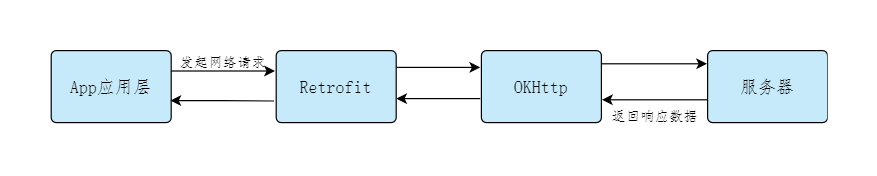
\includegraphics[width=.9\linewidth]{/software/retrofit}
    \caption{\label{fig:Retrofit}Retrofit的工作原理}
\end{figure}
Android客户端选择了Retrofit这一组件进行网络功能的开发。Retrofit是目前Android系统下最流行、应用最广的一个RESTful的HTTP网络请求框架的封装。
网络请求的工作本质上是OkHttp完成,而Retrofit仅负责网络请求接口的封装。
App应用程序通过Retrofit请求网络,实际上是使用Retrofit接口层封装请求参数、Header、URL等信息,之后由OkHttp完成后续的请求操作
在服务端返回数据之后,OkHttp将原始的结果交给Retrofit,Retrofit根据用户的需求对结果进行解析,这一过程如\autoref{fig:Retrofit}所示。

二、模型的上传

在前文中提及过的PE识别模型训练完成之后,得到的各机器学习模型也需要被上传部署在云服务器端。为使机器学习的部署更为便捷、清晰,软件系统也基于Python的图形界面PyQt额外开发了
机器学习模型上传程序,如\autoref{fig:upload_model}所示。而各机器学习模型在上传时,本质上仍使用了HTTP协议的POST方法。除\autoref{fig:upload_model}中已展示的外,
该POST方法在与云服务器端进行通讯时携带的全部参数及含义如\autoref{tab:post_paras2}所示,
其中文件类数据在表格中用粉红色底色进行了突出显示。
\begin{figure}[htbp]
    \centering
    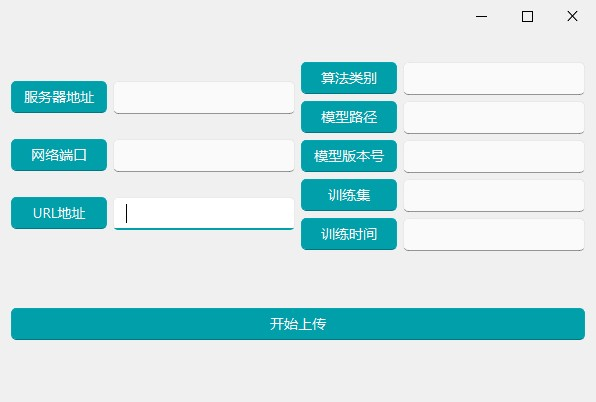
\includegraphics[width=.6\linewidth]{software/upload_model}
    \caption{\label{fig:upload_model}模型上传软件操作界面示意}
\end{figure}
\begin{longtblr}
    [
        theme                   = {zju},
        caption                 = {客户端在POST方法中上传的所有参数},
        label                   = {tab:post_paras2},
    ]
    {
        width                   = \linewidth,
        colspec                 = {X[1.5,c,m]X[3,c,m]X[1,c,m]X[1,c,m]X[2.5,c,m]},
        hline{1,Z}              = {\thickline},
        hline{2}                = {\thinline},
        rowhead                 = 1,
        row{odd}                = {bg=\oddcolor}, 
        row{even}               = {bg=\evencolor},
        row{1}                  = {font=\headfont,bg=\headcolor},
        row{2-Z}                = {font=\nonheadfont},
        cell{6}{3,4}            = {bg=\emphacolor},
    }
    参数的键名&参数值的含义&{数据流\\类型}&数据类型&备注\\
    project&上传的模型归属的具体项目&文本&字符串&{值固定为PE,代表数据隶属本论文基于PE的研究}\\
    data\_type&上传的模型所属生理信号类别&文本&字符串&{值固定为PPG}\\
    client&上传模型的客户端类型&文本&字符串&值固定为PC\\
    version&上传模型的客户端程序版本号&文本&字符串&\\
    model&训练生成得到的机器学习模型文件&文件&文件数据&模型导出为具体文件,按二进制编码成数据流发送\\
    model\_algorithm&模型训练生成所使用的机器学习算法&文本&字符串&包括KNN、RF等算法\\
    model\_version&使用特定机器学习算法生成的模型版本号&文本&字符串&\\
    train\_set&训练模型所使用的所有孕妇姓名&文本&字符串&{遵循医学伦理学相关标准,省略孕妇具体姓名,仅以拼音缩写代替}\\
    train\_time&模型训练生成时间&文本&字符串&\\
    upload\_time&本次通信上传时间&文本&字符串&\\
\end{longtblr}

三、基于Django的服务器端程序设计

为使云服务器端能对跨平台客户端的网络请求进行数据处理并作出响应,显然也需要进行云服务端程序的设计与开发。
而本研究涉及的所有机器学习模型均是通过Python下的Sklearn包生成,需要云服务器端也能处理、操作、使用这些经由互联网上传的机器学习模型。
因此,选用基于Python的Web框架进行云服务端程序的开发无疑是最为便捷的。

\begin{figure}[htbp]
    \centering
    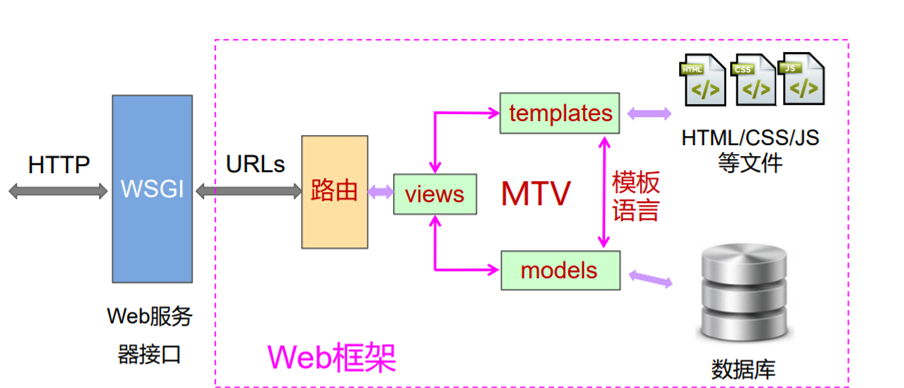
\includegraphics[width=.8\linewidth]{software/django}
    \caption{\label{fig:django}Django框架结构示意\cite{djangosq}}
\end{figure}
Django就是这样一个符合上述需求的、基于Python的开源通用Web框架,其整体结构如\autoref{fig:django}所示\cite{django,djangosq}。
Django免费开源,有活跃繁荣的社区以及丰富的文档,加上其本身由经验丰富的开发者构建,使得开发人员只需专注于编写应用程序,无需关注具体底层事务,从而可以快速开发安全和可维护的网站。
Django按模型-模版-视图(Model-Template-View,MTV)设计模式的进行了设计,MTV各自的职责与功能
如\autoref{tab:django_func}所示。
\begin{longtblr}
    [
        theme                   = {zju},
        caption                 = {Django框架的组成与功能},
        label                   = {tab:django_func},
    ]
    {
        width                   = \linewidth,
        colspec                 = {X[1,c,m]X[1,c,m]X[4,c,m]},
        hline{1,Z}              = {\thickline},
        hline{2}                = {\thinline},
        rowhead                 = 1,
        row{odd}                = {bg=\oddcolor}, 
        row{even}               = {bg=\evencolor},
        row{1}                  = {font=\headfont,bg=\headcolor},
        row{2-Z}                = {font=\nonheadfont},
        cell{6}{3,4}            = {bg=\emphacolor},
    }
    名称&层次&功能职责\\
    模型&数据存取层&处理与数据相关的所有事务:如何存取、如何验证有效性、包含哪些行为以及数据之间的关系等\\
    模板&表现层&处理与表现相关的决定:如何在页面或其他类型文档中进行显示\\
    视图&业务逻辑层&存取模型及调取恰当模板的相关逻辑。模型与模板的桥梁\\
\end{longtblr}

云服务器端的程序处理流程如\autoref{fig:url}所示。此前介绍过的\autoref{tab:post_paras}中的跨平台客户端的数据请求与\autoref{tab:post_paras2}中的
模型上传请求分别对应云服务器端的两个路由地址,即两个URL地址。对模型上传请求而言,云服务器端程序会在检查各项参数后,会在确认当前并无重复的算法及其版本后,将新的
模型存入数据库中供后续调用。而在处理跨平台客户端的数据请求时,程序也会进行参数检查,检查无误也会将所有数据进行存储。随后,依据数据请求中的是否需要进行数据预测参数,
数据请求中指定的需要使用的机器学习模型等参数,程序开始进行数据预测。由于本论文目前使用采集的数据量较小,当指定的机器学习模型被载入后,
程序会进一步检查,当前数据是否已经在模型训练阶段使用过,即当前数据是否在模型的训练集中。只有机器学习的未见数据实例才会被最终预测,同时,预测结果会被
返回至客户端。

以上介绍的处理流程实际上对应着\autoref{tab:django_func}中的视图,即业务逻辑层。而对于\autoref{tab:django_func}中的模板表现层而言,目前云服务器端程序对网络请求的处理较为简单,
只以纯文字的形式返回内容,没有进行专门的网页UI设计,故这部分不做过多介绍。而\autoref{tab:django_func}中的模型
\begin{figure}[h]
    \centering
    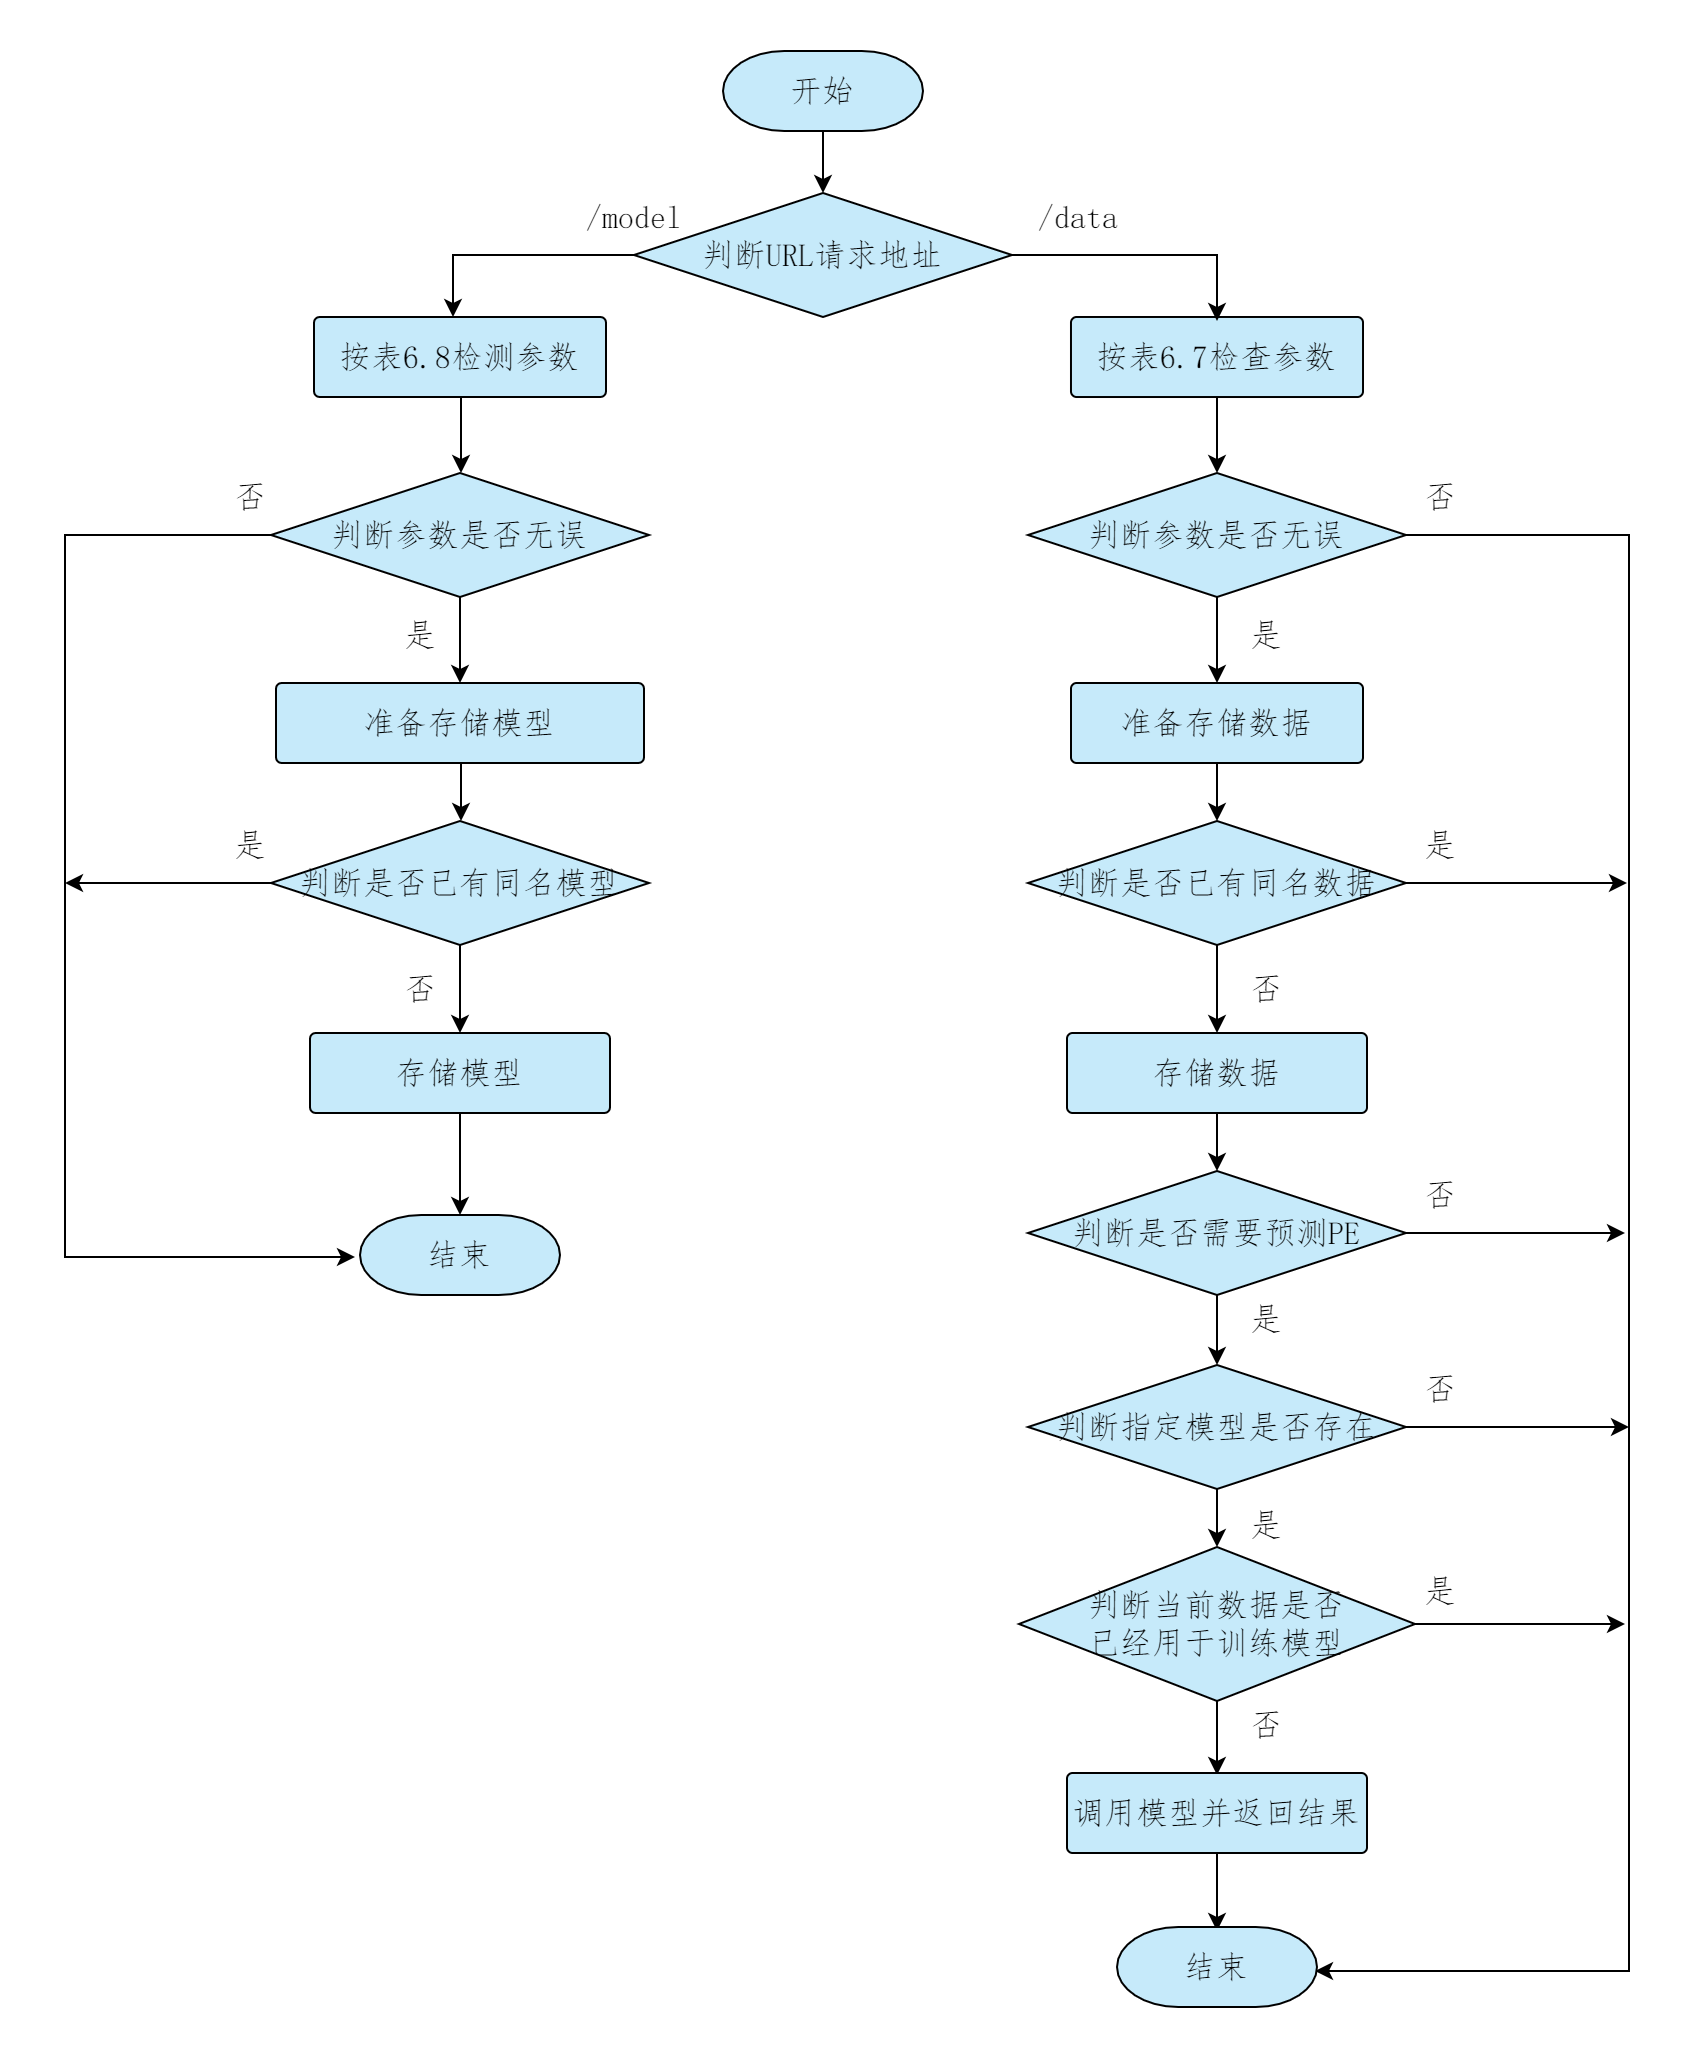
\includegraphics[width=0.8\linewidth]{software/url}
    \caption{\label{fig:url}云服务器响应URL请求过程流程图}
\end{figure}

\noindent
涉及了数据库的处理操作,这部分的程序设计会在后续进行介绍。

另外,为方便调试,云服务端在使用Django进行开发时,也启用了日志记录功能。由于这部分的程序功能也是基于Python下的logging包开发,具体过程与此前模型训练模块的类似,故不再单独赘述。

四、数据库设计

数据库(DataBase, DB)是按照数据结构来组织、存储和管理数据的仓库,也是一个长期存储在计算机内的、有组织的、可共享的、统一管理的大量数据的集合。
经过多年的发展,数据库技术已经是现代互联网数据管理的基本方法和技术,在组织数据、维护数据、控制数据和利用数据等方面发挥着不可替代的重要作用,
是计算机领域最重要的基础软件之一,也是确保计算机系统稳定运行的基石。

另一方面,关系型数据库是对存储的格式能够直观地反映实体间的关系的一类数据库的统称。关系型数据库和常见的表格比较相似,数据库的表与表之间是有很多复杂的关联关系。
而MySQL就是一种最为常见、也最具代表性的关系型数据库,也是目前流行的主流关系数据库之一。
MySQL遵循结构化查询语言(Structured Query Language,SQL)标准,支持查询、新增、更新、删除、求和、排序等基本操作。
为使云服务器端的数据管理更为便捷有效,同时应对后续可能的大量数据管理,综合软件系统的开发过程中也基于MySQL进行了简单的数据库设计。

数据库中的数据一词指数据库可以储存多种信息,这些信息一般被称为字段。而为了从包含多条数据记录的集合中获取特定记录,还必须从这些字段中定义主键(PRIMARY KEY)。
主键通常可以是一个字段或多个字段的组合,其值能唯一地标识表中的每一行,通过它可强制表的实体完整性。主键在与其他表的外键关联以及数据记录的修改与删除中具有重要作用。

另一方面,如前所述,不论是如\autoref{tab:post_paras}上传的数据请求还是如\autoref{tab:post_paras2}上传的模型请求,都包含了大量参数信息,这些信息必须进行高效、有序的完整储存。
与此同时,相比模型请求而言,数据请求中的参数种类常常会随着软件系统的迭代而发生较大的改变,比如数据信号种类的变更,PPG特征的增改等。这也要求软件系统在进行数据库设计时,必须同时
保持一定的兼容性设计。

\begin{figure}[htbp]
    \centering
    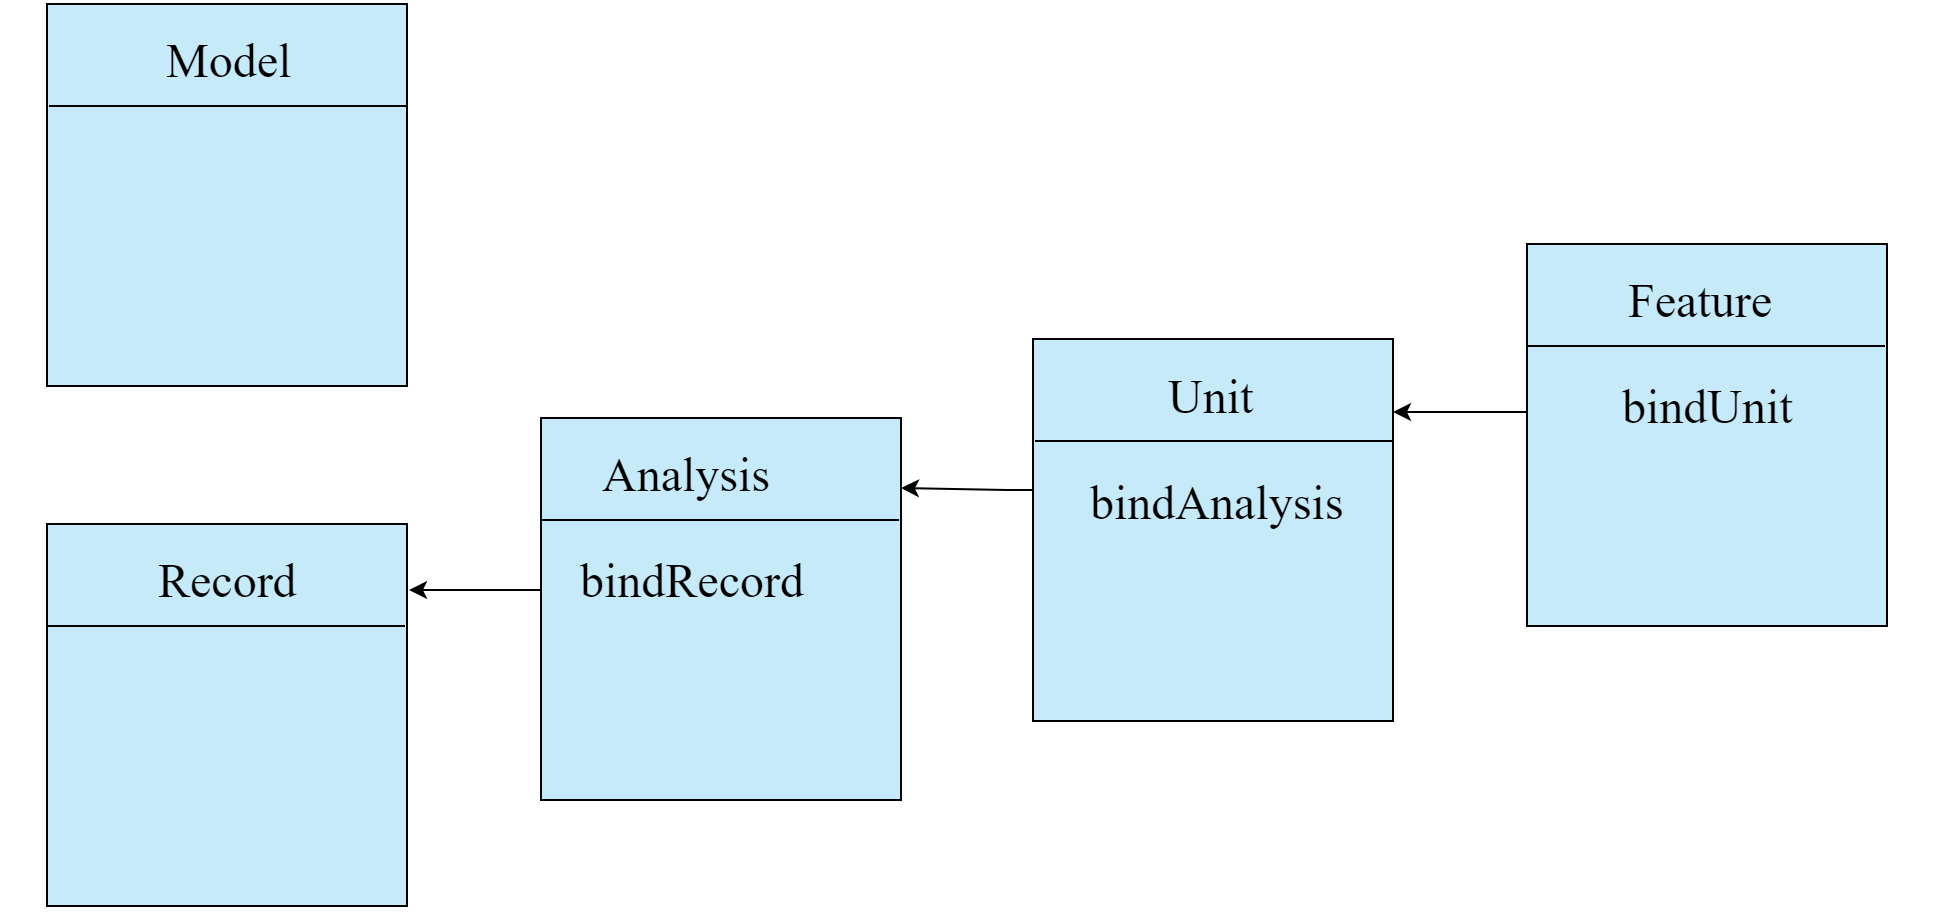
\includegraphics[width=.8\linewidth]{software/data_table_relationship}
    \caption{\label{fig:data_table_relationship}软件系统的数据表及数据关系示意图}
\end{figure}

基于以上考虑,软件系统最终设计了多张数据表(Table)以管理存储客户端上传来的数据与模型文件。这些数据表之间的相互关联关系如\autoref{fig:data_table_relationship}所示。
可以看到,模型的存储过程较为简单;而相对地,为保证兼容性,生理信号数据及其衍生特征的存储较为复杂,需要多张数据表级联并相互配合。
需要注意的是,为简明扼要,\autoref{fig:data_table_relationship}中仅显示了各数据表的重要的外部键,这些数据表的详细设计可参见
\autoref{tab:data_table_record}至\autoref{tab:data_table_model}。
\begin{longtblr}
    [
        theme                   = {zju},
        caption                 = {Record数据表的字段设计},
        label                   = {tab:data_table_record},
    ]
    {
        width                   = \linewidth,
        colspec                 = {X[1,c,m]X[1,c,m]X[2,c,m]X[2,c,m]},
        hline{1,Z}              = {\thickline},
        hline{2}                = {\thinline},
        rowhead                 = 1,
        row{odd}                = {bg=\oddcolor}, 
        row{even}               = {bg=\evencolor},
        row{1}                  = {font=\headfont,bg=\headcolor},
        row{2-Z}                = {font=\nonheadfont},
        cell{2}{4}              = {bg=\emphacolor},
    }
    字段&数据类型&意义&备注\\
    AutoField&32位整型&自增字段&Django默认主键,随记录存储自动增加\\
    project&字符串&数据归属项目&兼容性设计,默认值为PE\\
    sourceFileName&字符串&上传的原始数据文件名&\\
    sourceFile&字符串&上传的原始数据文件&Django会自动管理文件名与文件的映射关系\\
    person&字符串&原始数据文件来源的人名&\\
    state&状态变量&整型&兼容性设计,在PE项目中指代用户PE患病状态,0为健康,1为PE,2为PE待定;其他项目中state意义可根据需要自定义\\
    sampleTime&字符串&数据采集时间&\\
    createTime&时间日期&当前Record存储时间&时间日期为Django自定义的数据类型\\
    isDeleted&布尔量&当前记录是否被逻辑“删除”&为避免记录被直接物理删除,额外增加的布尔变量指代是否被删除状态\\
\end{longtblr}

\begin{longtblr}
    [
        theme                   = {zju},
        caption                 = {Analysis数据表的字段设计},
        label                   = {tab:data_table_analysis},
    ]
    {
        width                   = \linewidth,
        colspec                 = {X[1,c,m]X[2,c,m]X[3,c,m]X[4,c,m]},
        hline{1,Z}              = {\thickline},
        hline{2}                = {\thinline},
        rowhead                 = 1,
        row{odd}                = {bg=\oddcolor}, 
        row{even}               = {bg=\evencolor},
        row{1}                  = {font=\headfont,bg=\headcolor},
        row{2-Z}                = {font=\nonheadfont},
        cell{2-3}{4}            = {bg=\emphacolor},
    }
    字段&数据类型&意义&备注\\
    AutoField&32位整型&自增字段&Django默认主键,随记录存储自动增加\\
    bindRecord&\autoref{tab:data_table_record}中定义的Record记录&当前记录绑定的Record数据表记录ID&关联到Record数据表的外部键\\
    dataType&字符串&数据记录所属类别&兼容性设计,在PE项目中,可选值包括指代特征的feature与指代原始采用点的point\\
    dataVersion&字符串&上传的数据特征文件版本号&兼容性设计,保持软件系统对因算法迭代导致的数据调整的兼容\\
    jsonFile&字符串&上传的数据特征文件&Django会自动管理文件名与文件的映射关系\\
    createTime&时间日期&当前Record存储时间&时间日期为Django自定义的数据类型\\
    isDeleted&布尔量&当前记录是否被逻辑“删除”&为避免记录被直接物理删除,额外增加的布尔变量指代是否被删除状态\\
\end{longtblr}

\begin{longtblr}
    [
        theme                   = {zju},
        caption                 = {Unit数据表的字段设计},
        label                   = {tab:data_table_unit},
    ]
    {
        width                   = \linewidth,
        colspec                 = {X[1,c,m]X[2,c,m]X[3,c,m]X[4,c,m]},
        hline{1,Z}              = {\thickline},
        hline{2}                = {\thinline},
        rowhead                 = 1,
        row{odd}                = {bg=\oddcolor}, 
        row{even}               = {bg=\evencolor},
        row{1}                  = {font=\headfont,bg=\headcolor},
        row{2-Z}                = {font=\nonheadfont},
        cell{2-3}{4}            = {bg=\emphacolor},
    }
    字段&数据类型&意义&备注\\
    AutoField&32位整型&自增字段&Django默认主键,随记录存储自动增加\\
    bindAnalysis&\autoref{tab:data_table_analysis}中定义的Analysis记录&当前记录绑定的Analysis数据表记录ID&关联到Analysis数据表的外部键\\
    signalType&字符串&数据类型&兼容性设计,在PE项目中,目前该值仅为PPG\\
    index&整型&最小分析单位编号&兼容性设计,在PE项目中,该值指代PPG原始记录中的完整波形序号\\
    isDeleted&布尔量&当前记录是否被逻辑“删除”&为避免记录被直接物理删除,额外增加的布尔变量指代是否被删除状态\\
\end{longtblr}

\begin{longtblr}
    [
        theme                   = {zju},
        caption                 = {Feature数据表的字段设计},
        label                   = {tab:data_table_feature},
    ]
    {
        width                   = \linewidth,
        colspec                 = {X[1,c,m]X[2,c,m]X[3,c,m]X[4,c,m]},
        hline{1,Z}              = {\thickline},
        hline{2}                = {\thinline},
        rowhead                 = 1,
        row{odd}                = {bg=\oddcolor}, 
        row{even}               = {bg=\evencolor},
        row{1}                  = {font=\headfont,bg=\headcolor},
        row{2-Z}                = {font=\nonheadfont},
        cell{2-3}{4}            = {bg=\emphacolor},
    }
    字段&数据类型&意义&备注\\
    AutoField&32位整型&自增字段&Django默认主键,随记录存储自动增加\\
    bindUnit&\autoref{tab:data_table_unit}中定义的Unit记录&当前记录绑定的Unit数据表记录ID&关联到Unit数据表的外部键\\
    type&字符串&操作标记&兼容性设计,在PE项目组,对PPG的特征类数值无意义;对PPG的采样点数据记录的均一化等特性\\
    name&字符串&特征数据名称&兼容性设计,特征名。在PE项目组,特征类数据该值为具体特征缩写;对采样点数据该值固定为point\\
    value&Json&具体特征值&兼容性设计,Django支持直接以Json形式存储字段信息\\
    isDeleted&布尔量&当前记录是否被逻辑“删除”&为避免记录被直接物理删除,额外增加的布尔变量指代是否被删除状态\\
\end{longtblr}

\begin{longtblr}
    [
        theme                   = {zju},
        caption                 = {Model数据表的字段设计},
        label                   = {tab:data_table_model},
    ]
    {
        width                   = \linewidth,
        colspec                 = {X[1,c,m]X[2,c,m]X[3,c,m]X[4,c,m]},
        hline{1,Z}              = {\thickline},
        hline{2}                = {\thinline},
        rowhead                 = 1,
        row{odd}                = {bg=\oddcolor}, 
        row{even}               = {bg=\evencolor},
        row{1}                  = {font=\headfont,bg=\headcolor},
        row{2-Z}                = {font=\nonheadfont},
        cell{2}{4}              = {bg=\emphacolor},
    }
    字段&数据类型&意义&备注\\
    AutoField&32位整型&自增字段&Django默认主键,随记录存储自动增加\\
    model&字符串&机器学习模型文件&Django会自动管理文件名与文件的映射关系\\
    algorithm&字符串&机器学习训练使用的算法名称&\\
    version&字符串&模型的版本号&兼容性设计,支持模型版本更迭\\
    trainSet&Json&记录当前模型训练所使用的用户数据&\\
    trainTime&字符串&记录模型训练时间&\\
    uploadTime&字符串&记录模型上传时间&\\
    isDeleted&布尔量&当前记录是否被逻辑“删除”&为避免记录被直接物理删除,额外增加的布尔变量指代是否被删除状态\\
\end{longtblr}
\section{测试与验证}
此前的内容主要对软件系统的功能的设计与实现进行了介绍,在软件开发完成后,还需要对其各项模块功能与最终完整功能进行一定的实际验证。本小节将对这部分的工作进行介绍。

\subsection{算法测试与验证}
数据预处理模块的验证主要集中在对本研究设计提出的SCD波形检测算法的验证与测试上。

\subsection{多客户端一致性的测试与验证}

\subsection{网络连接的测试与验证}

\subsection{预测模型的测试与验证}

\section{小结}
